\documentclass[a4paper,11pt]{article}
\usepackage[polish]{babel}
\usepackage[utf8]{inputenc}   % lub utf8
\usepackage[T1]{fontenc}
\usepackage{graphicx}
\usepackage{anysize}
\usepackage{enumerate}
\usepackage{times}
 
%\marginsize{left}{right}{top}{bottom}
\marginsize{3cm}{3cm}{3cm}{3cm}
\setlength{\parindent}{1em}
\sloppy

\usepackage{enumitem}
\setlist[enumerate,1]{label=\arabic*}
\setlist[enumerate,2]{label=\theenumi.\arabic*}
\setlist[enumerate,3]{label=\theenumii.\arabic*}

\title{Inżynieria Oprogramowania - analiza systemu aquaparku}
\date{2019/20}
\author{Piotr Wawrzynów \and Wojciech Dolata} 

\begin{document}

\newcommand{\pspec}[4]{#1 \\wejście: #2 \\wyjście: #3 \\działanie: #4}

\maketitle
\newpage



\tableofcontents
\newpage


 
\section{Streszczenie systemu}
Modelowany przez nas system w całości obsługuje aquapark. Posiada on możliwość prowadzenia transakcji kupna biletu jednorazowego oraz karnetów okresowych zarówno na miejscu, jak i on-line. Klient po założeniu konta na stronie internetowej może za jej pomocą zakupić karnet, który jest na stałe przypisany do konta (karty). Płatność internetowa odbywa się za pomocą pośrednika oferującego obsługę takich płatności. Na terenie basenu, przy kasie istnieje możliwość płatności kartą lub gotówką. Jednym z zadań systemu jest również obsługa księgowości, czyli między innymi wystawianie faktur dla podwykonawców (np. firma ratownicza, firma sprzątająca), rozliczanie podatku VAT.\\ \\
System umożliwia również korzystanie z usług firmy gastronomicznej, której za pewną kwotę udostępnia się wydzielone miejsce na terenie aquaparku. Firma zapewniająca bezpieczeństwo w wodzie dostarcza wykwalifikowaną kadrę ratowniczą. W systemie instruktor prowadzi lekcje pływania dla dzieci i młodzieży. Aquapark na potrzeby lekcji rezerwuje tor w basenie, na którym instruktor prowadzi zajęcia doskonalące technikę pływania, lub pojedynczy basen, w którym odbywają się zajęcia aerobiku. Dodatkowo możliwa jest indywidualna rezerwacja toru, za dodatkową opłatą.
\newpage


\section{Obiekty}
\begin{itemize}
    \item Klient - osoba korzystająca z usług aquaparku
    \item Pracownicy aquaparku
            \begin{itemize}
                \item Kasjer - osoba przyjmująca wpłaty i wydająca bilety wstępu
                \item Instruktor - nauczyciel pływania
                \item Księgowy - osoba zajmująca się szeroko pojętymi finansami
                \item Szatniarz - osoba odpowiedzialna za obsługę szatni
                \item Kierownik - osoba zatrudniająca firmy zewnętrzne
            \end{itemize}
    \item Narzędzia informatyczne
            \begin{itemize}
                \item strona internetowa - pozwala na otrzymanie informacji związanych z aquaparkiem oraz zakup biletu on-line
                \item program rozliczający - kalkuluje cenę biletu przy wstępie (system punktowy) lub przy wyjściu (system czasowy)
            \end{itemize}
    \item Firmy zewnętrzne
            \begin{itemize}
                \item firma sprzątająca
                \item firma obsługująca gastronomię
                \item firma obsługująca płatności internetowe (np. przelewy 24)
                \item firma ratownicza (np. WOPR)
            \end{itemize}
\end{itemize}



\section{Zdarzenia}
\begin{itemize}
    \item założenie konta stałego klienta
    \item zakup biletu jednorazowego lub karnetu
            \begin{itemize}
                \item on-line
                \item osobiście
            \end{itemize}
    \item rezerwacja toru (np. przez naukę pływania)
    \item wykupienie lekcji pływania
    \item uiszczenie płatności
    \item wybór sposobu płatności
            \begin{itemize}
                \item gotówka
                \item karta
            \end{itemize}
\end{itemize}
\newpage


\section{Diagram kontekstowy}
    \begin{figure}[!htb]
    \centerline{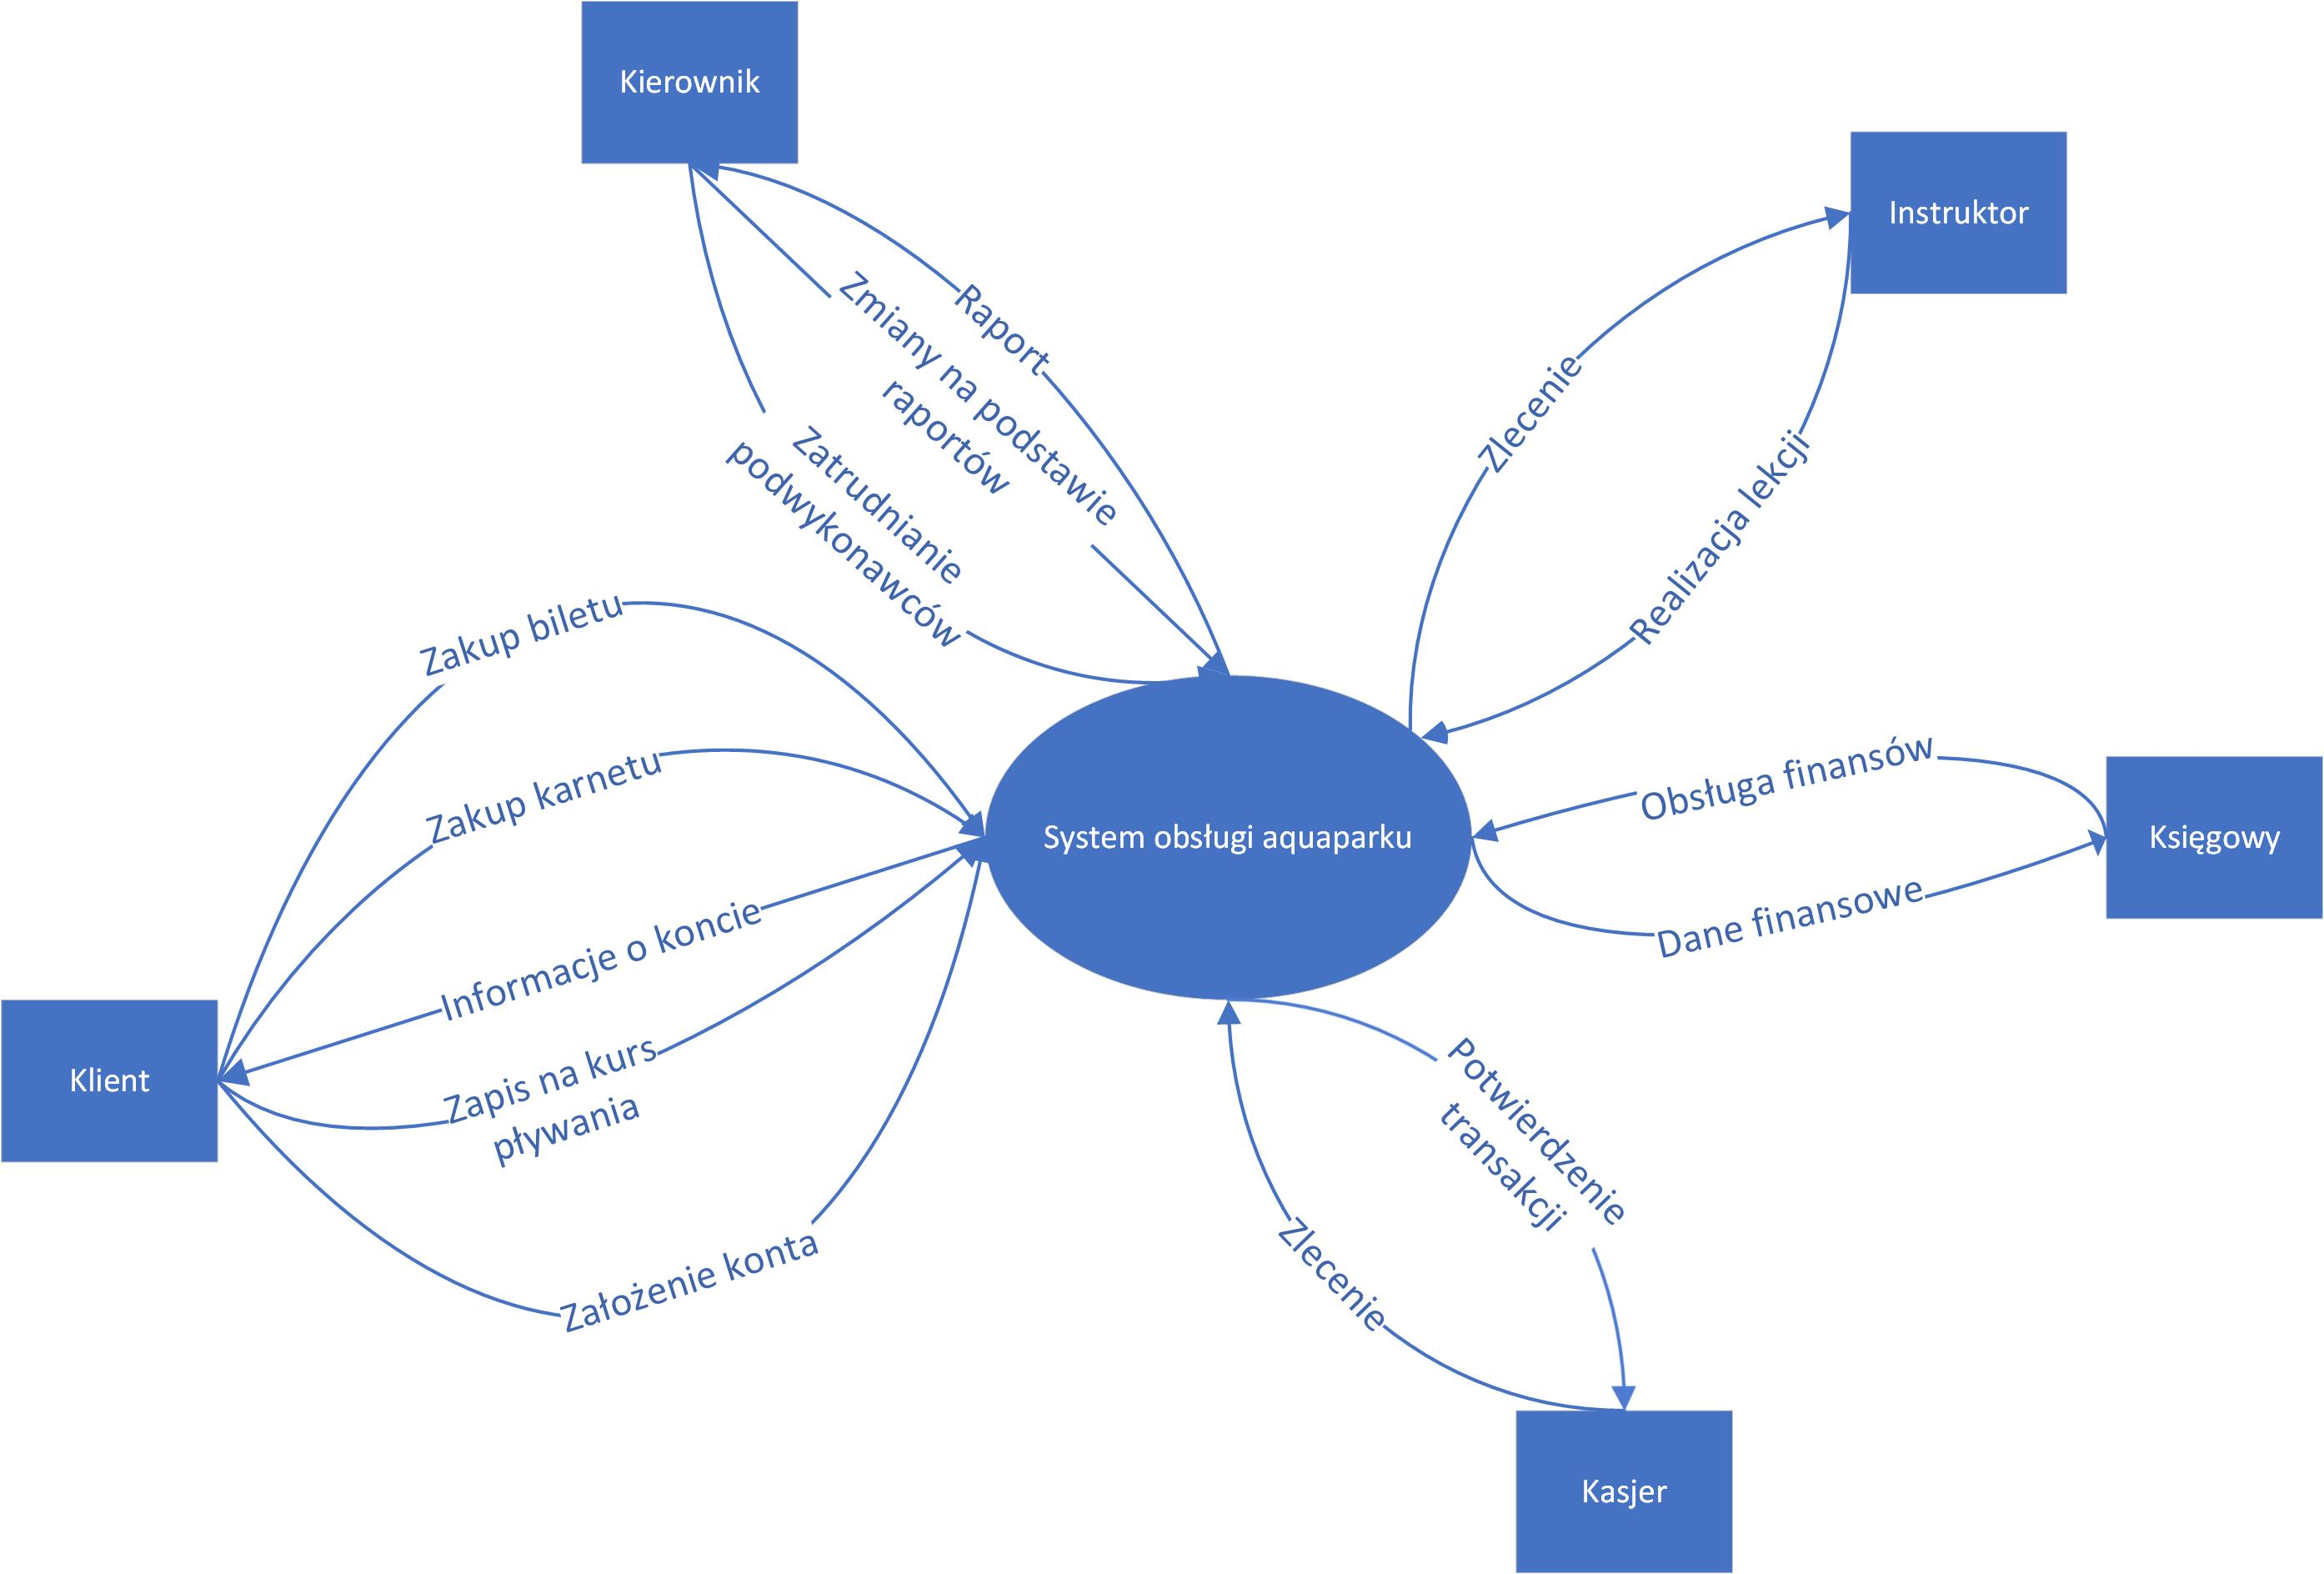
\includegraphics[scale=0.7]{kontekstowy.jpg}}
    \label{fig:kontekstowy}
    \end{figure}
\newpage



\section{Diagramy DFD}
\subsection{Poziom 0}
    \begin{figure}[!htb]
    \centerline{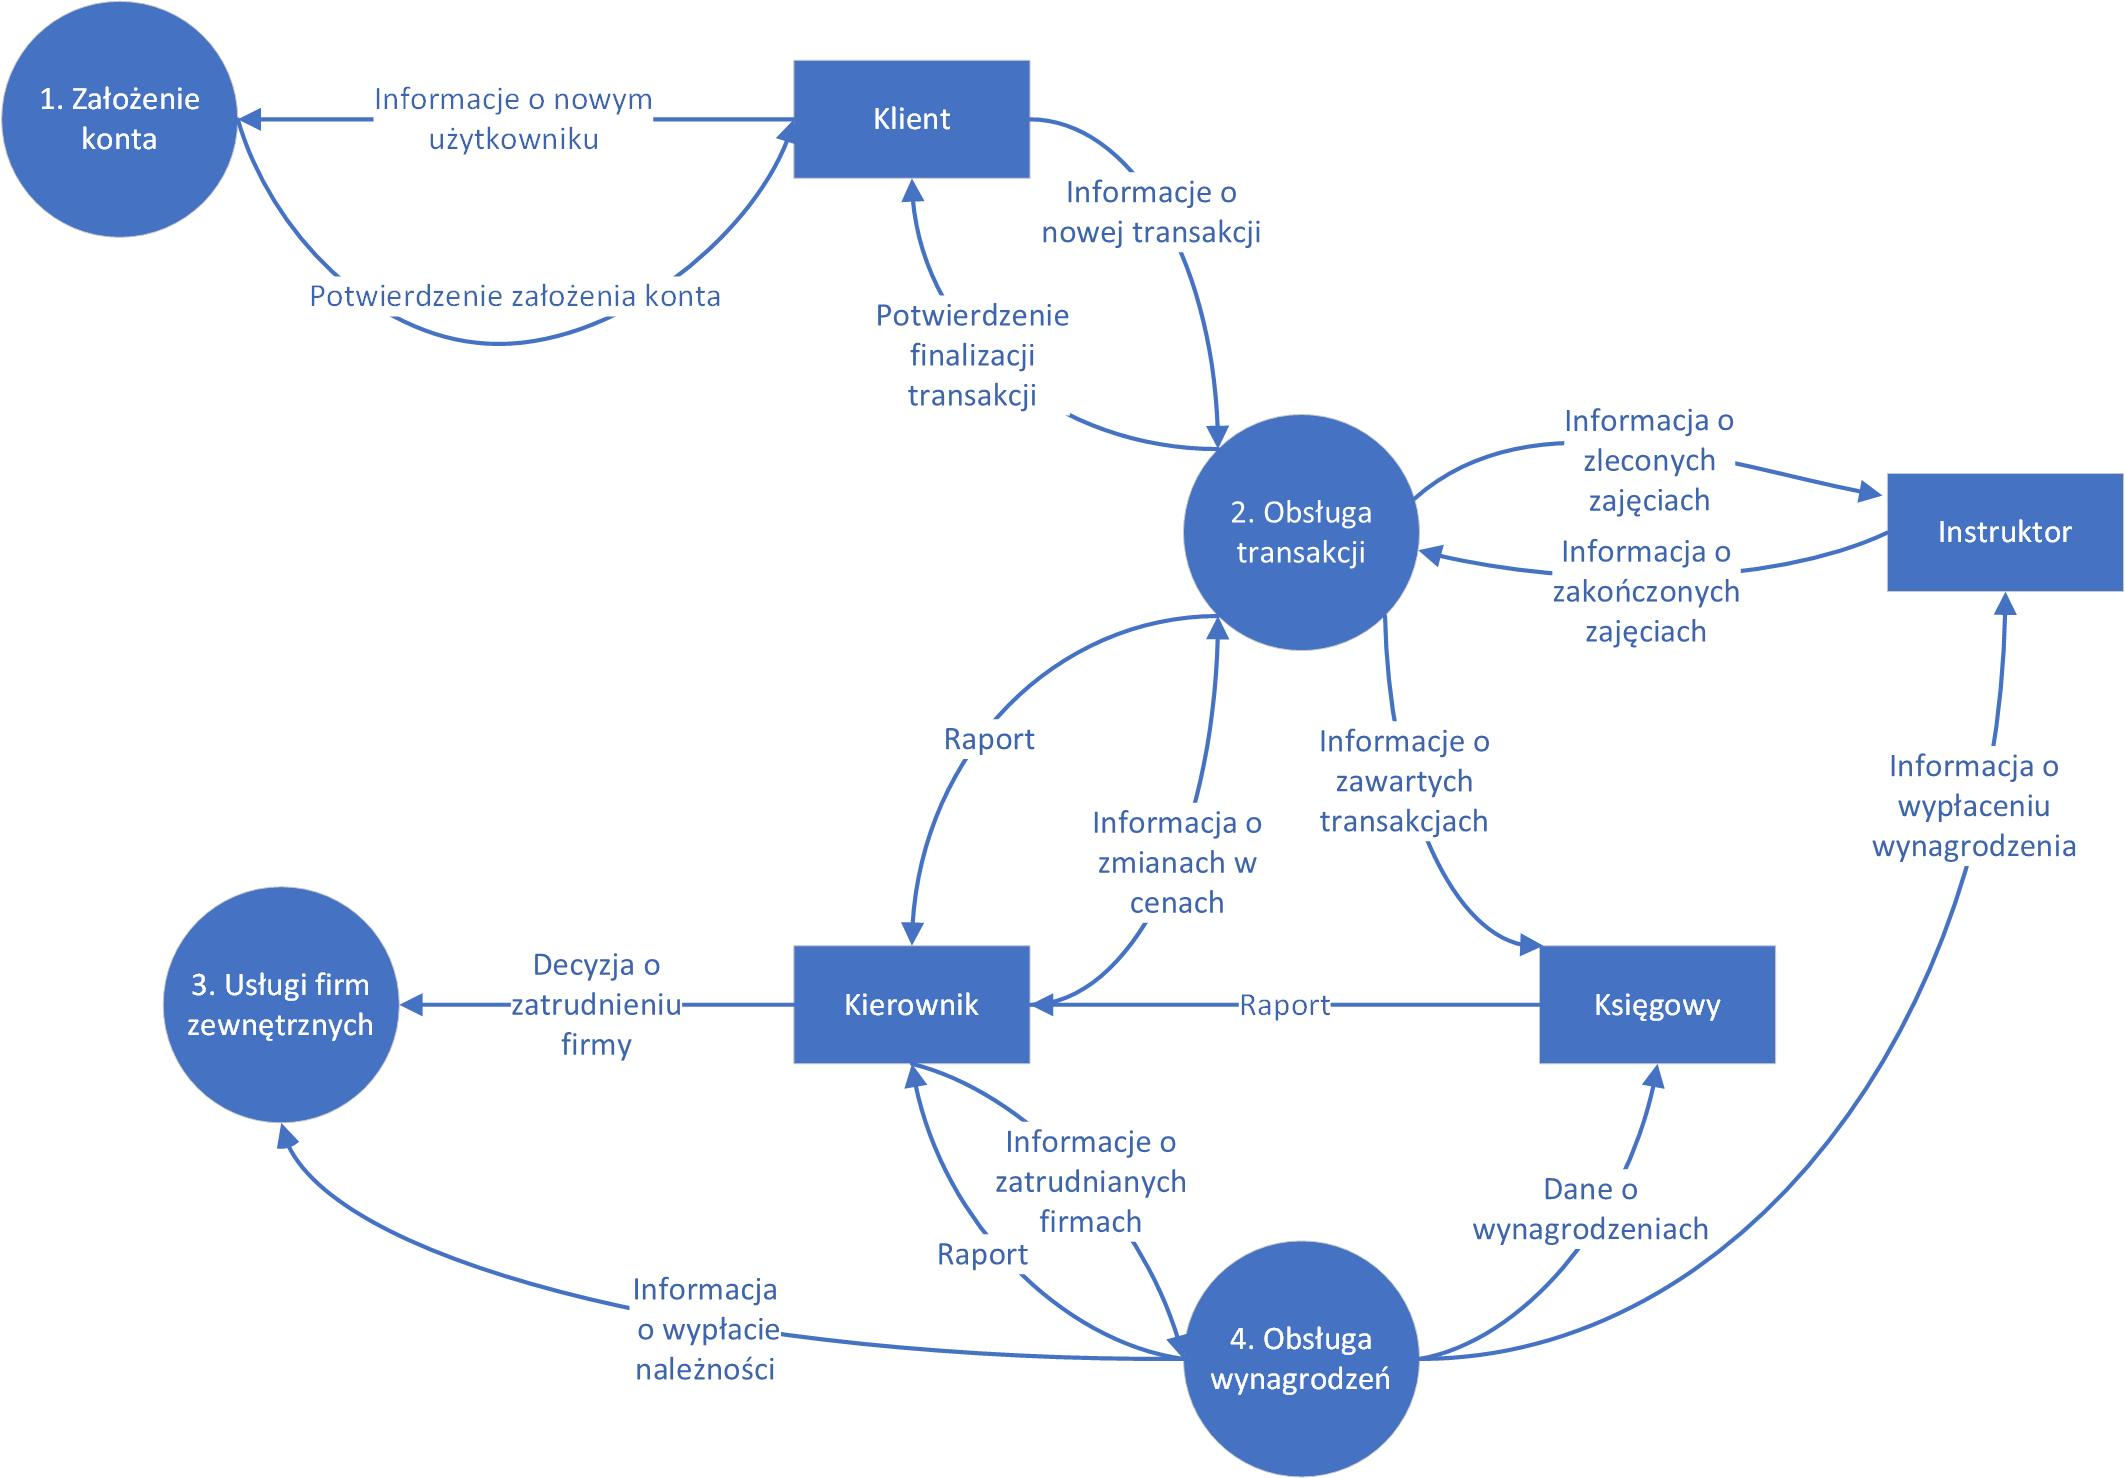
\includegraphics[scale=0.9]{level0.jpg}}
    \label{fig:level0}
    \end{figure}
\newpage



\subsection{Poziom 1}
\subsubsection{Dekompozycja procesu Założenie konta}
    \begin{figure}[!htb]
    \centerline{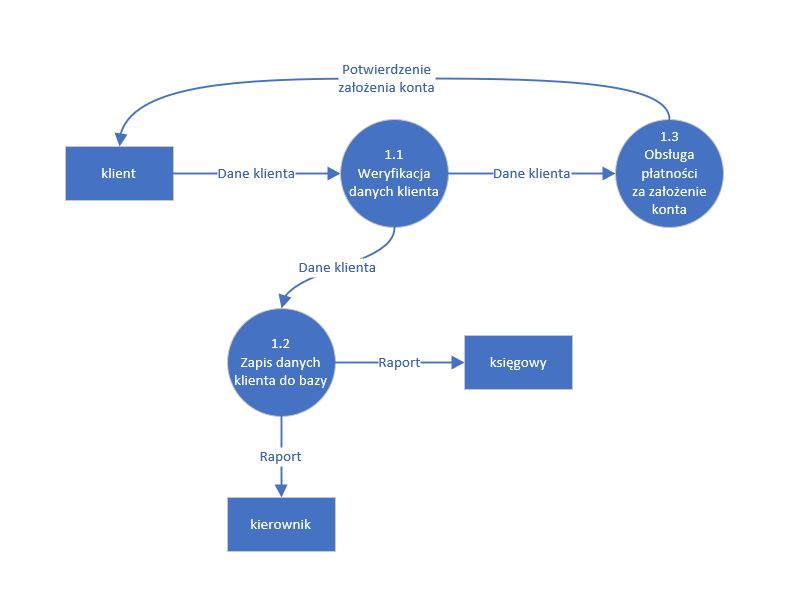
\includegraphics[scale=0.8]{level1_1.jpg}}
    \label{fig:level1_1}
    \end{figure}
    \newpage



\subsubsection{Dekompozycja procesu Obsługa transakcji}
    \begin{figure}[!htb]
    \centerline{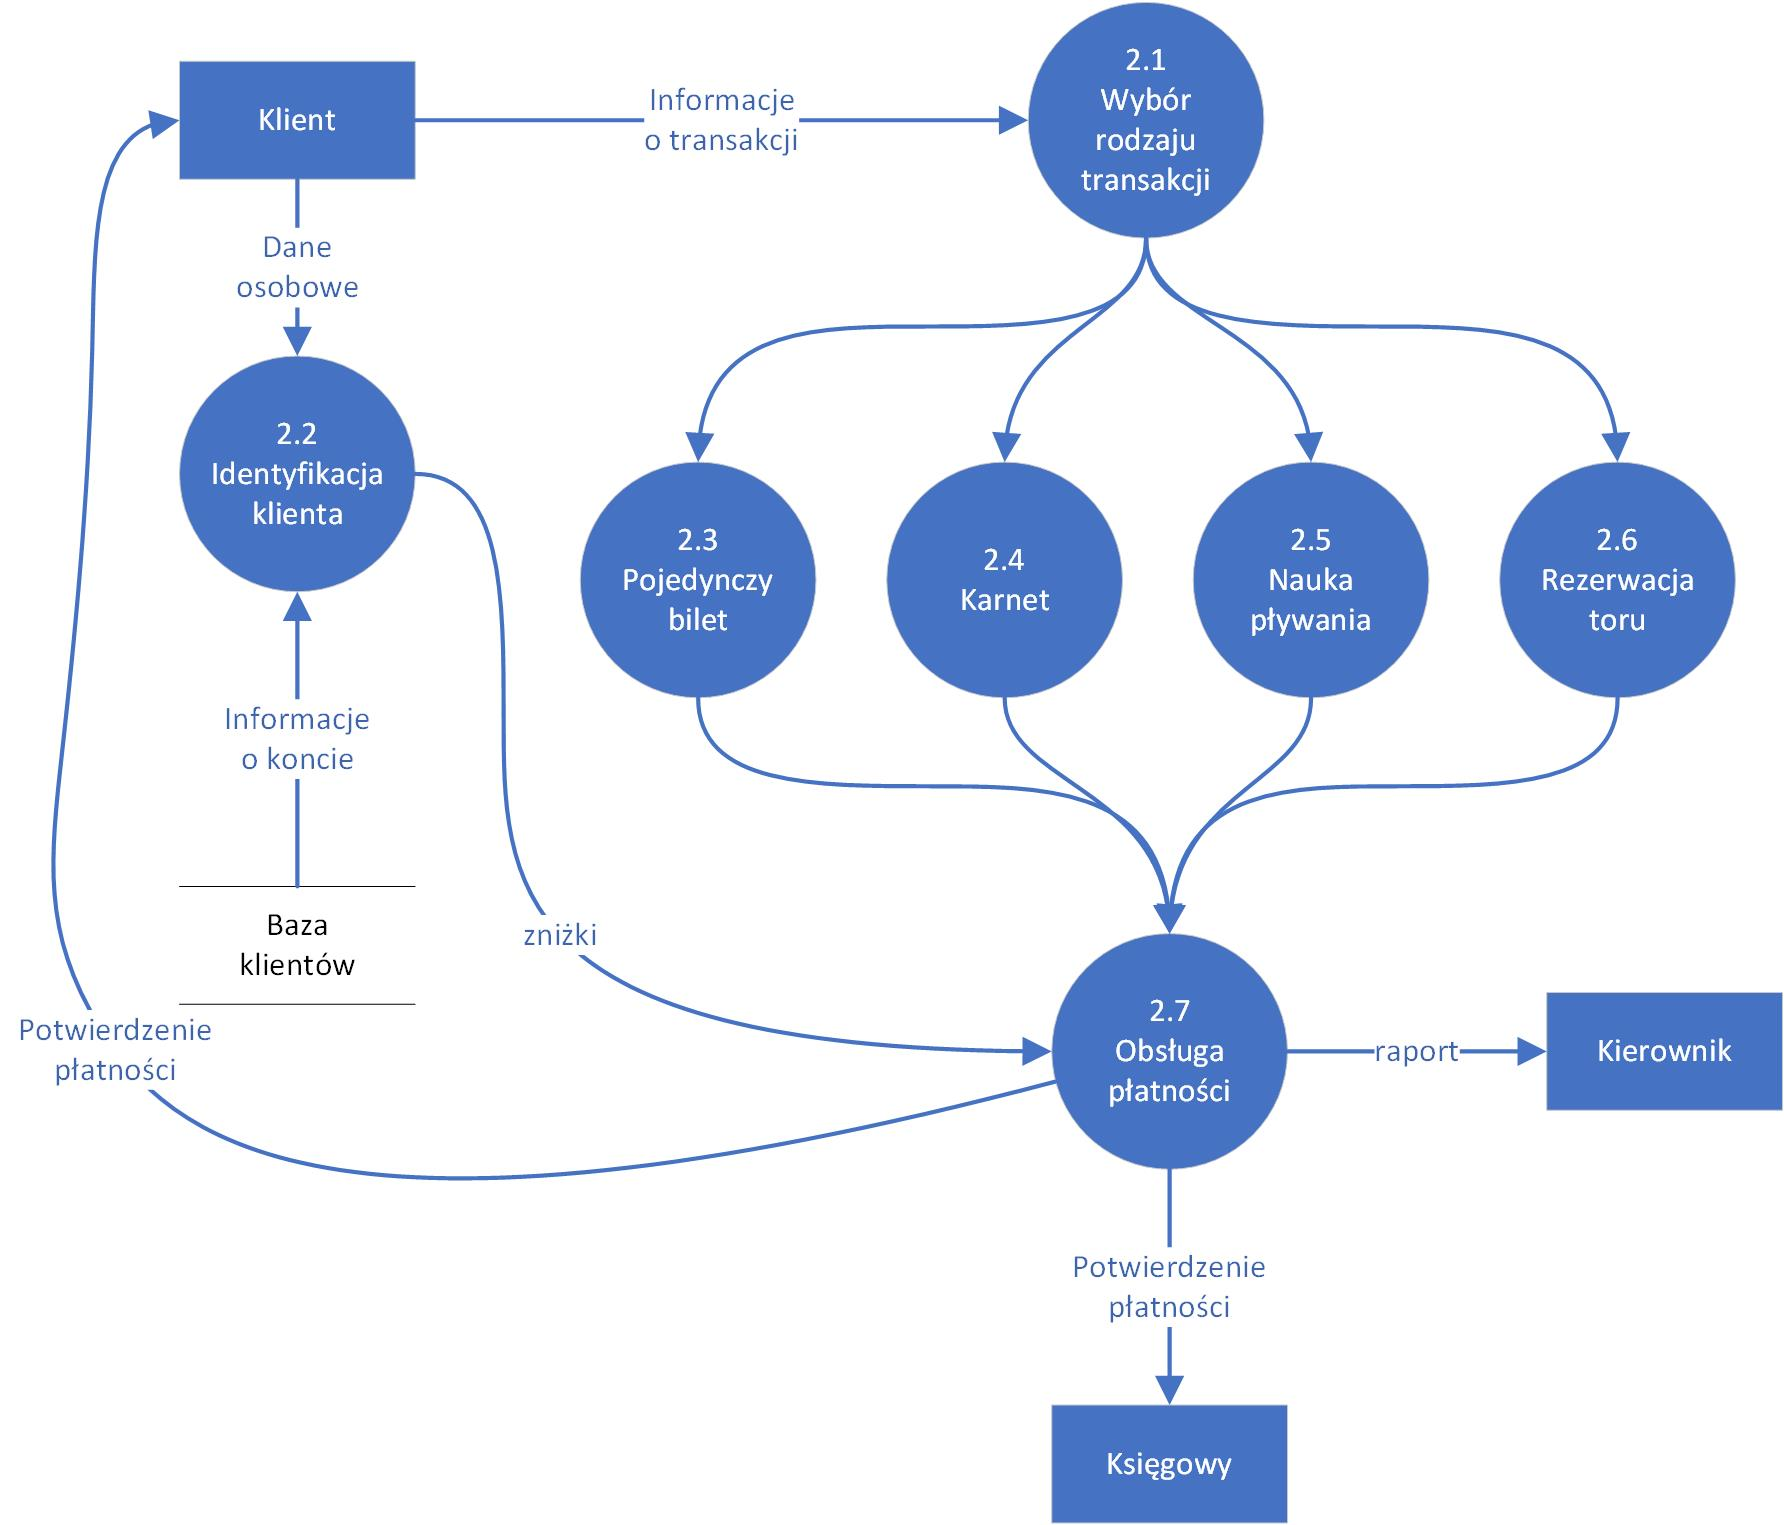
\includegraphics[scale=1.1]{level1_2.jpg}}
    \label{fig:level1_2}
    \end{figure}
    \newpage



\subsubsection{Dekompozycja procesu Usługi firm zewnętrznych}
    \begin{figure}[!htb]
    \centerline{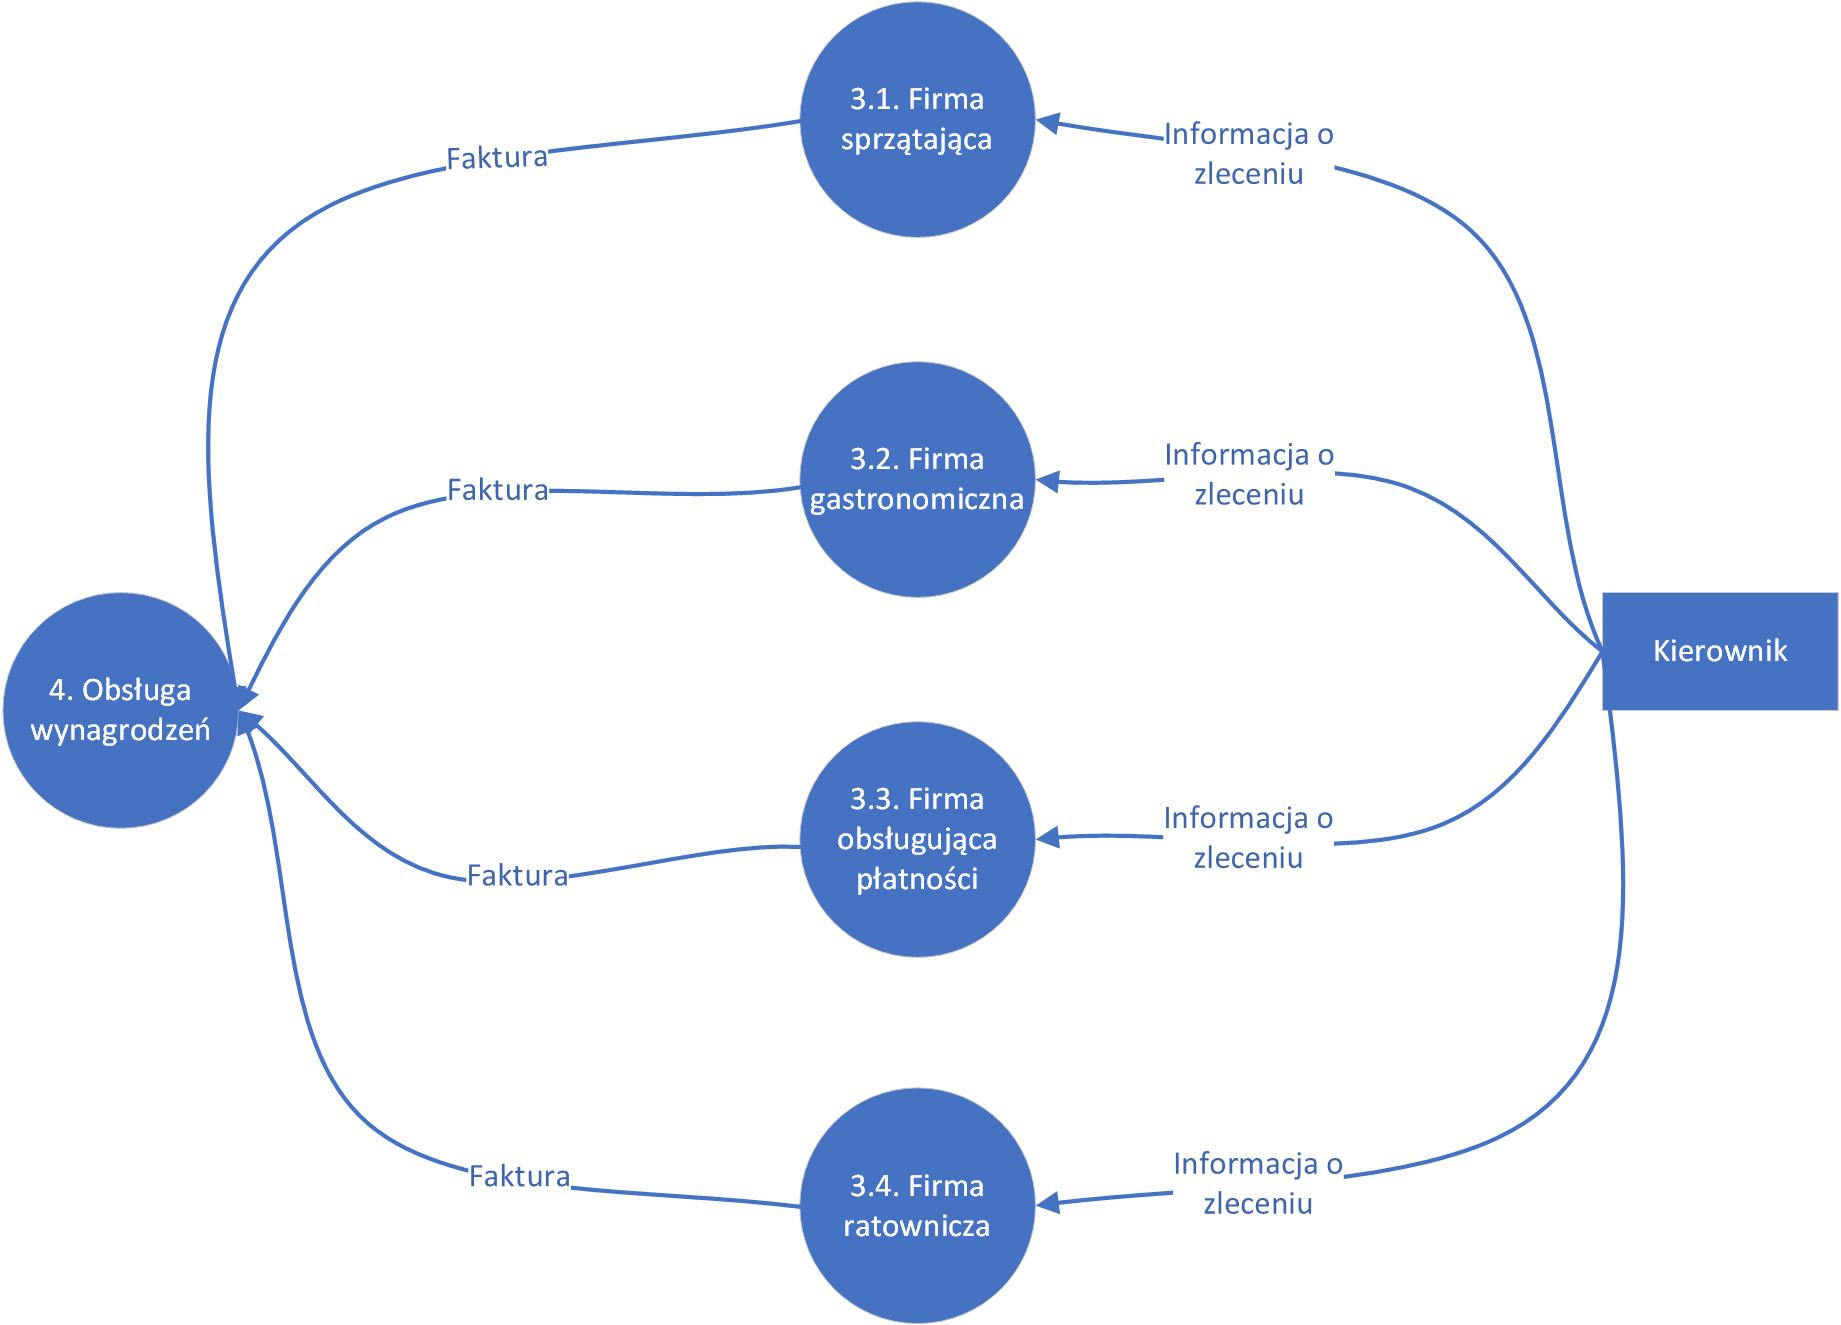
\includegraphics[scale=1.1]{level1_3.jpg}}
    \label{fig:level1_3}
    \end{figure}
    \newpage
  
\subsubsection{Dekompozycja procesu Obsługa wynagrodzeń}
    \begin{figure}[!htb]
    \centerline{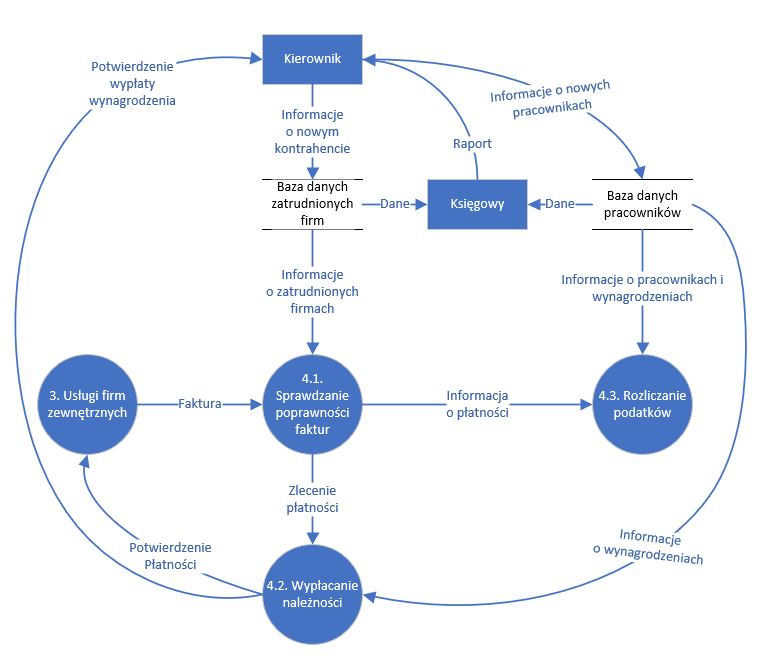
\includegraphics[scale=0.8]{level1_4.jpg}}
    \label{fig:level1_4}
    \end{figure}
    \newpage  
    
    
    
\subsection{Poziom 2}
\subsubsection{Dekompozycja procesu Weryfikacja danych klienta}
    \begin{figure}[!htb]
    \centerline{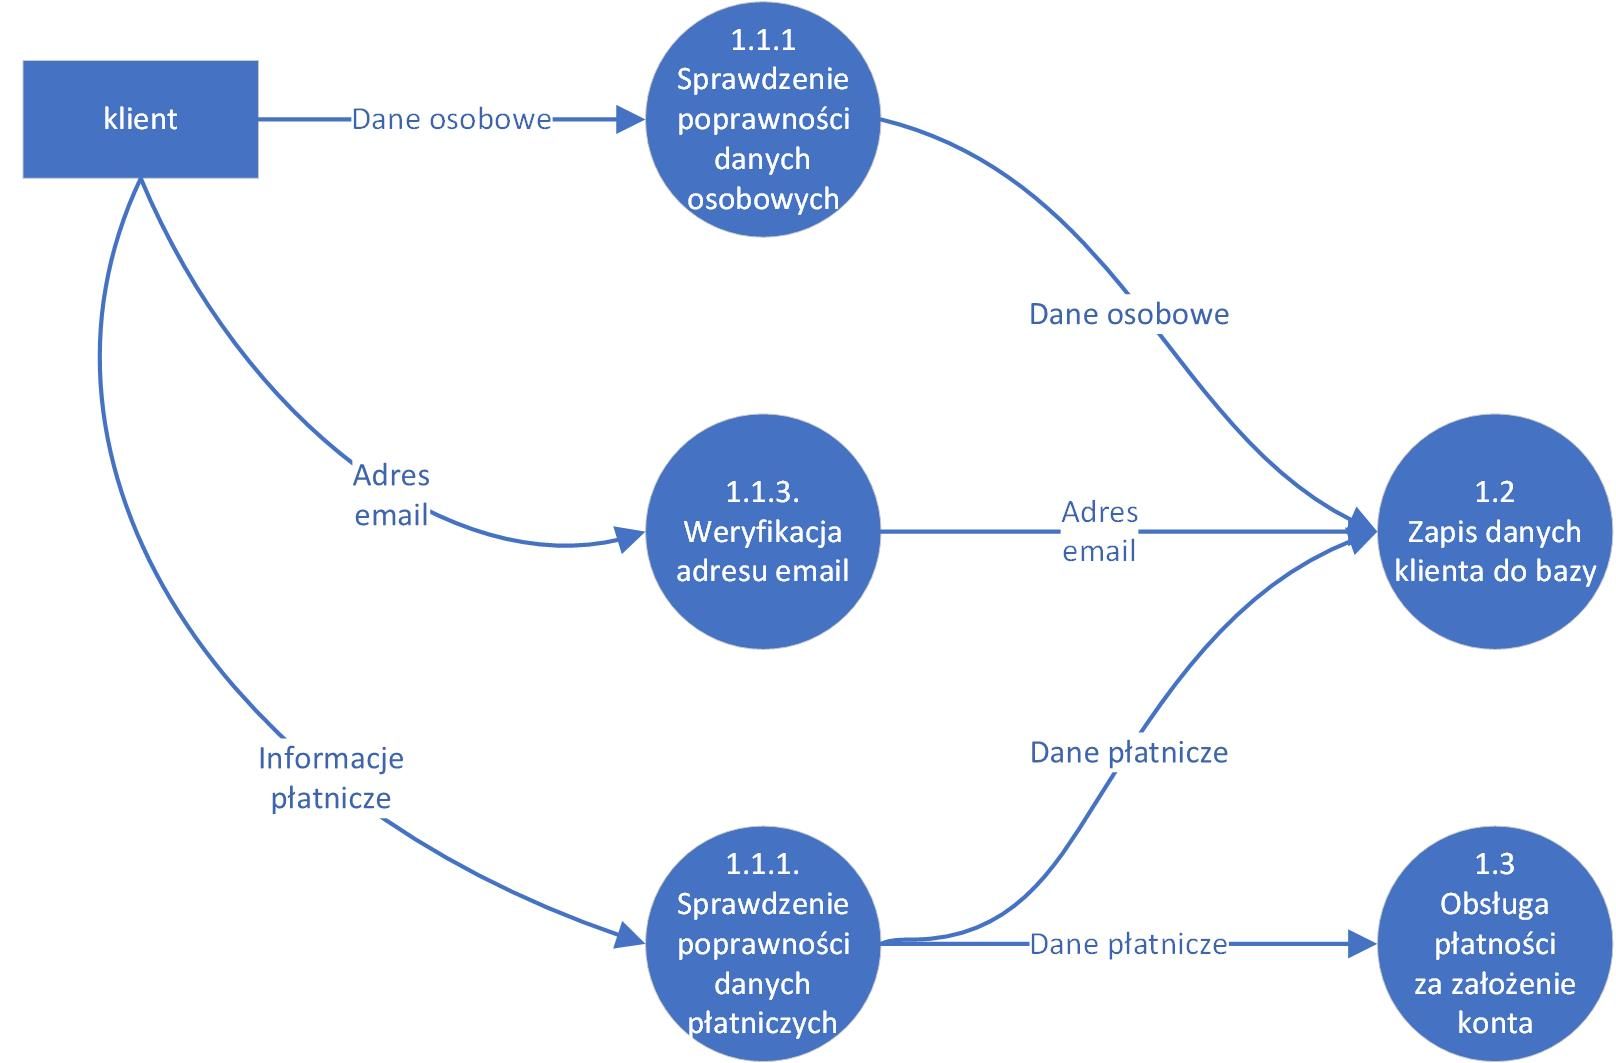
\includegraphics[scale=1.1]{level2_1_1.jpg}}
    \label{fig:level2_1_1}
    \end{figure}
    \newpage
    
\subsubsection{Dekompozycja procesu Zapis danych klienta do bazy}
    \begin{figure}[!htb]
    \centerline{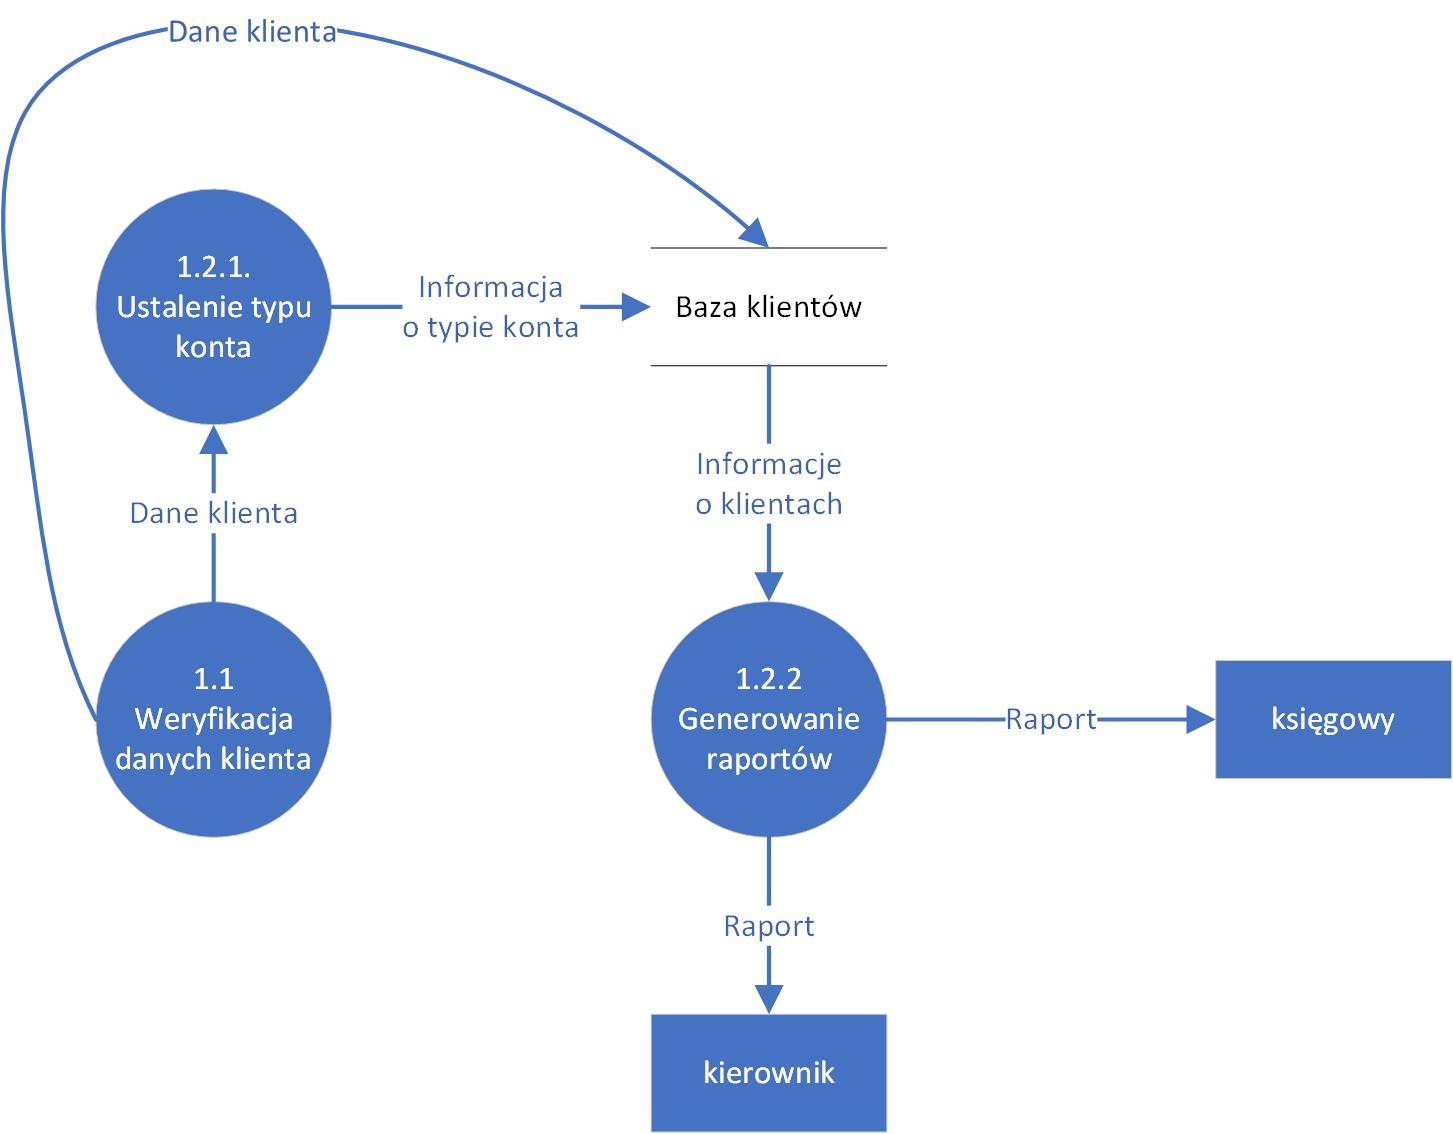
\includegraphics[scale=1.1]{level2_1_2.jpg}}
    \label{fig:level2_1_2}
    \end{figure}
    \newpage
    
\subsubsection{Dekompozycja procesu Obsługa płatności za założenie konta}
    \begin{figure}[!htb]
    \centerline{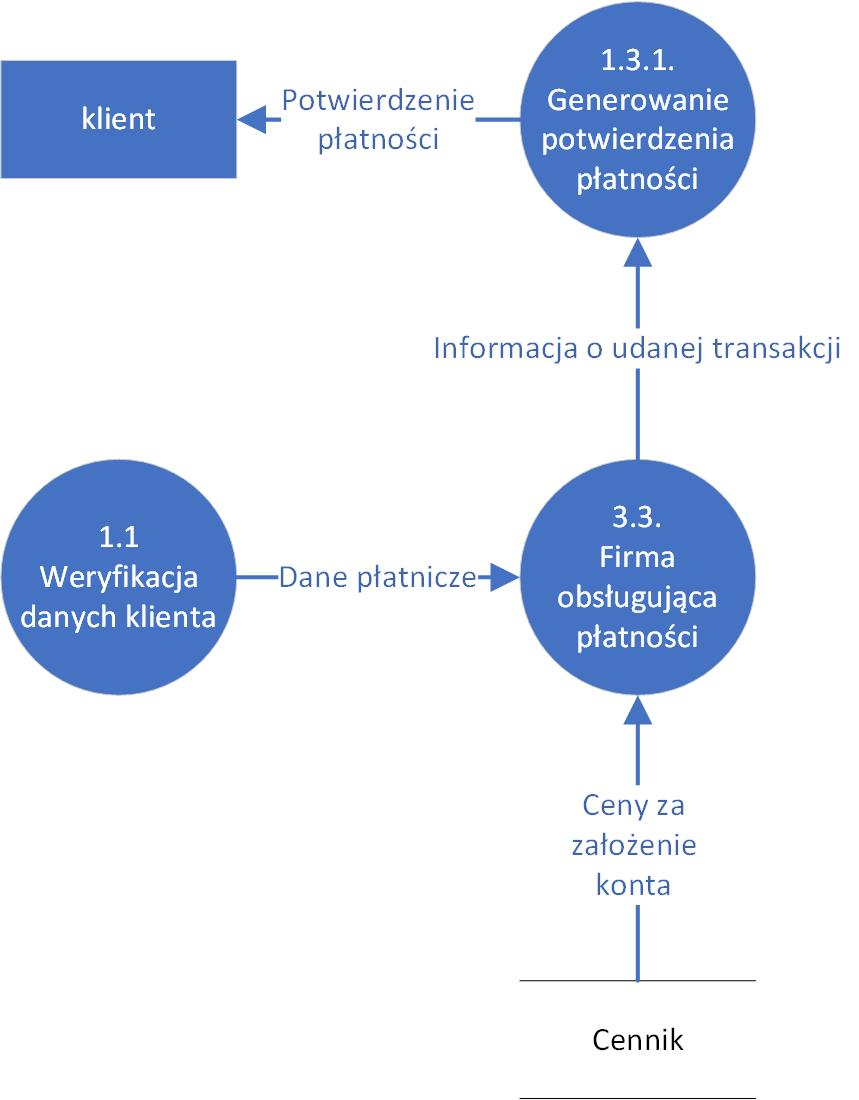
\includegraphics[scale=1.1]{level2_1_3.jpg}}
    \label{fig:level2_1_3}
    \end{figure}
    \newpage
    
\subsubsection{Dekompozycja procesu Pojedynczy bilet}
    \begin{figure}[!htb]
    \centerline{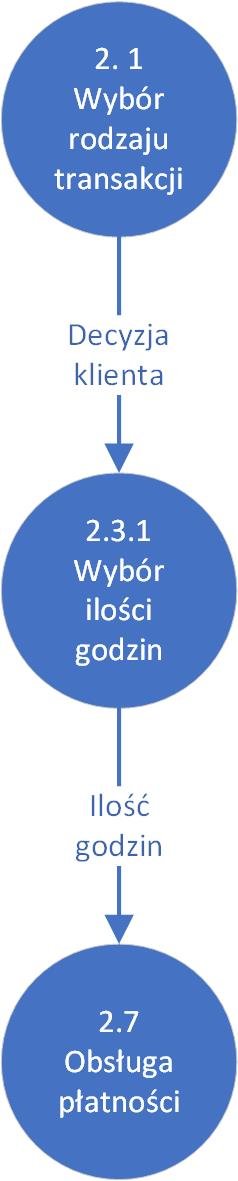
\includegraphics[scale=1.1]{level2_2_3.jpg}}
    \label{fig:level2_2_3}
    \end{figure}
    \newpage
    
\subsubsection{Dekompozycja procesu Karnet}
    \begin{figure}[!htb]
    \centerline{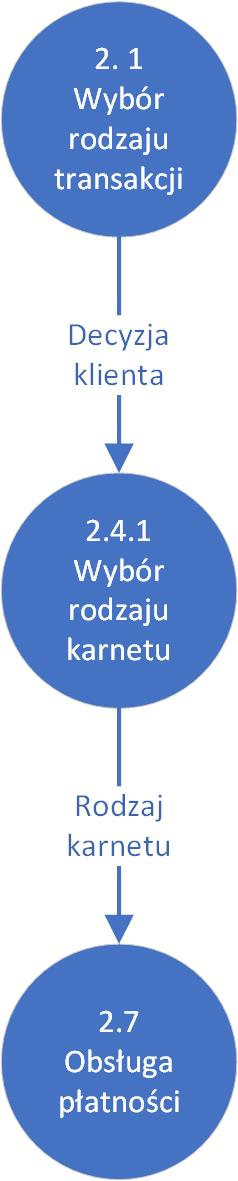
\includegraphics[scale=1.1]{level2_2_4.jpg}}
    \label{fig:level2_2_4}
    \end{figure}
    \newpage
    
\subsubsection{Dekompozycja procesu Nauka pływania}
    \begin{figure}[!htb]
    \centerline{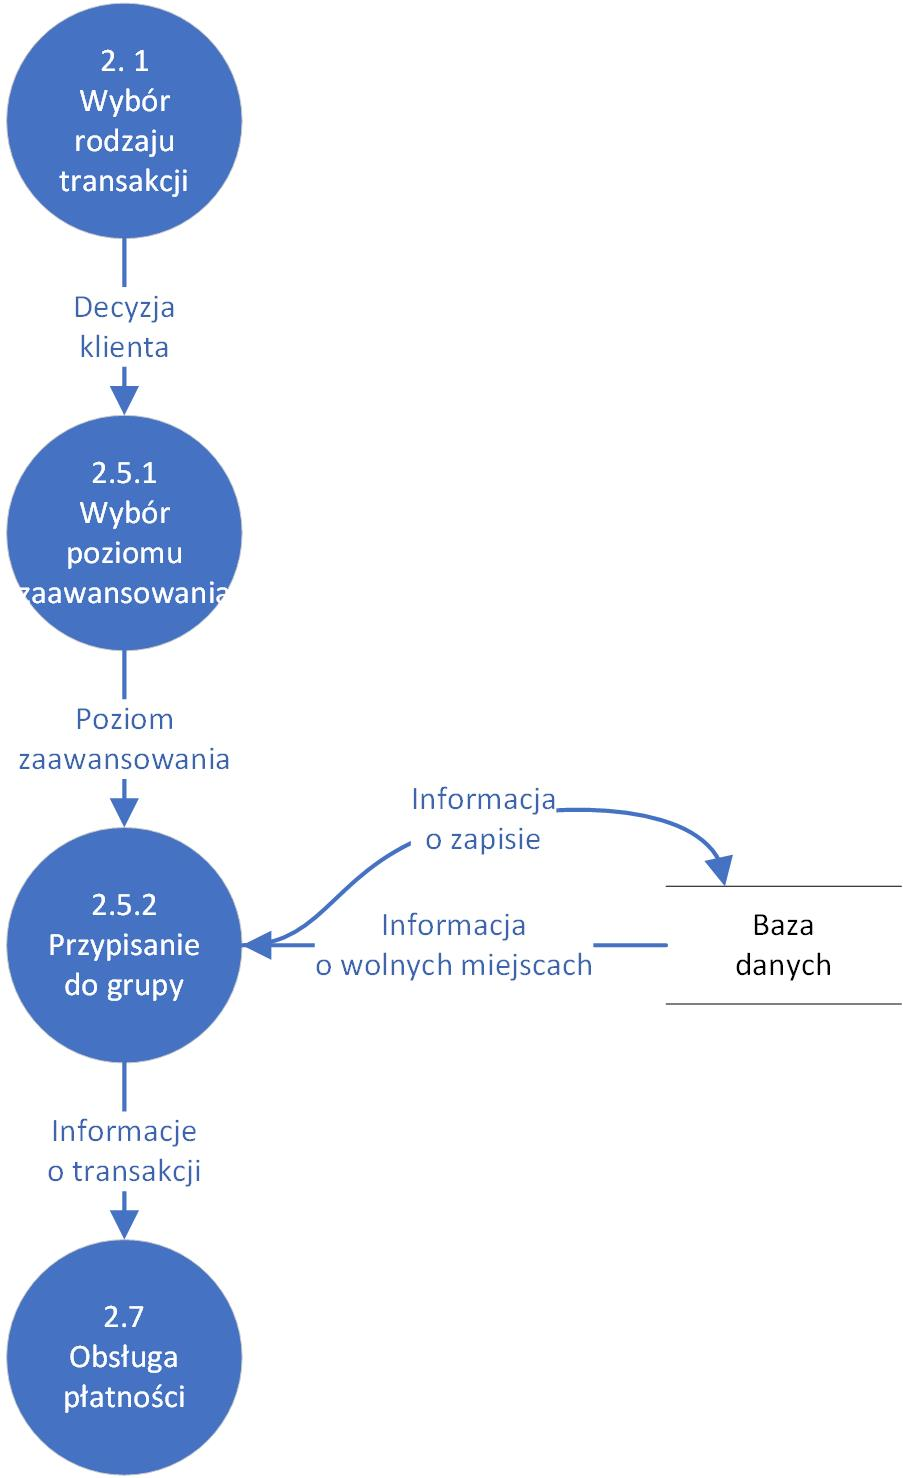
\includegraphics[scale=1.1]{level2_2_5.jpg}}
    \label{fig:level2_2_5}
    \end{figure}
    \newpage
    
\subsubsection{Dekompozycja procesu Rezerwacja toru}
    \begin{figure}[!htb]
    \centerline{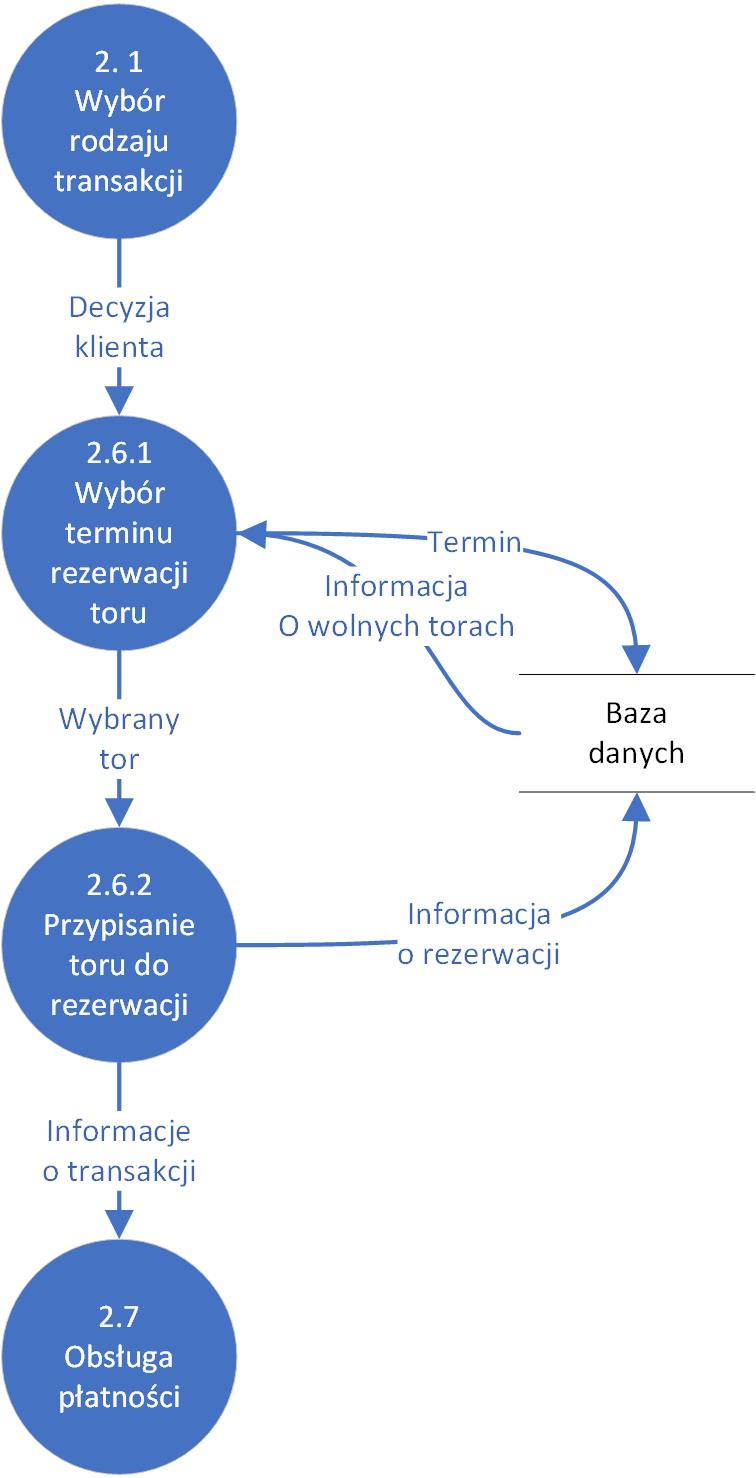
\includegraphics[scale=1.1]{level2_2_6.jpg}}
    \label{fig:level2_2_6}
    \end{figure}
    \newpage
    
\subsubsection{Dekompozycja procesu Obsługa płatności}
    \begin{figure}[!htb]
    \centerline{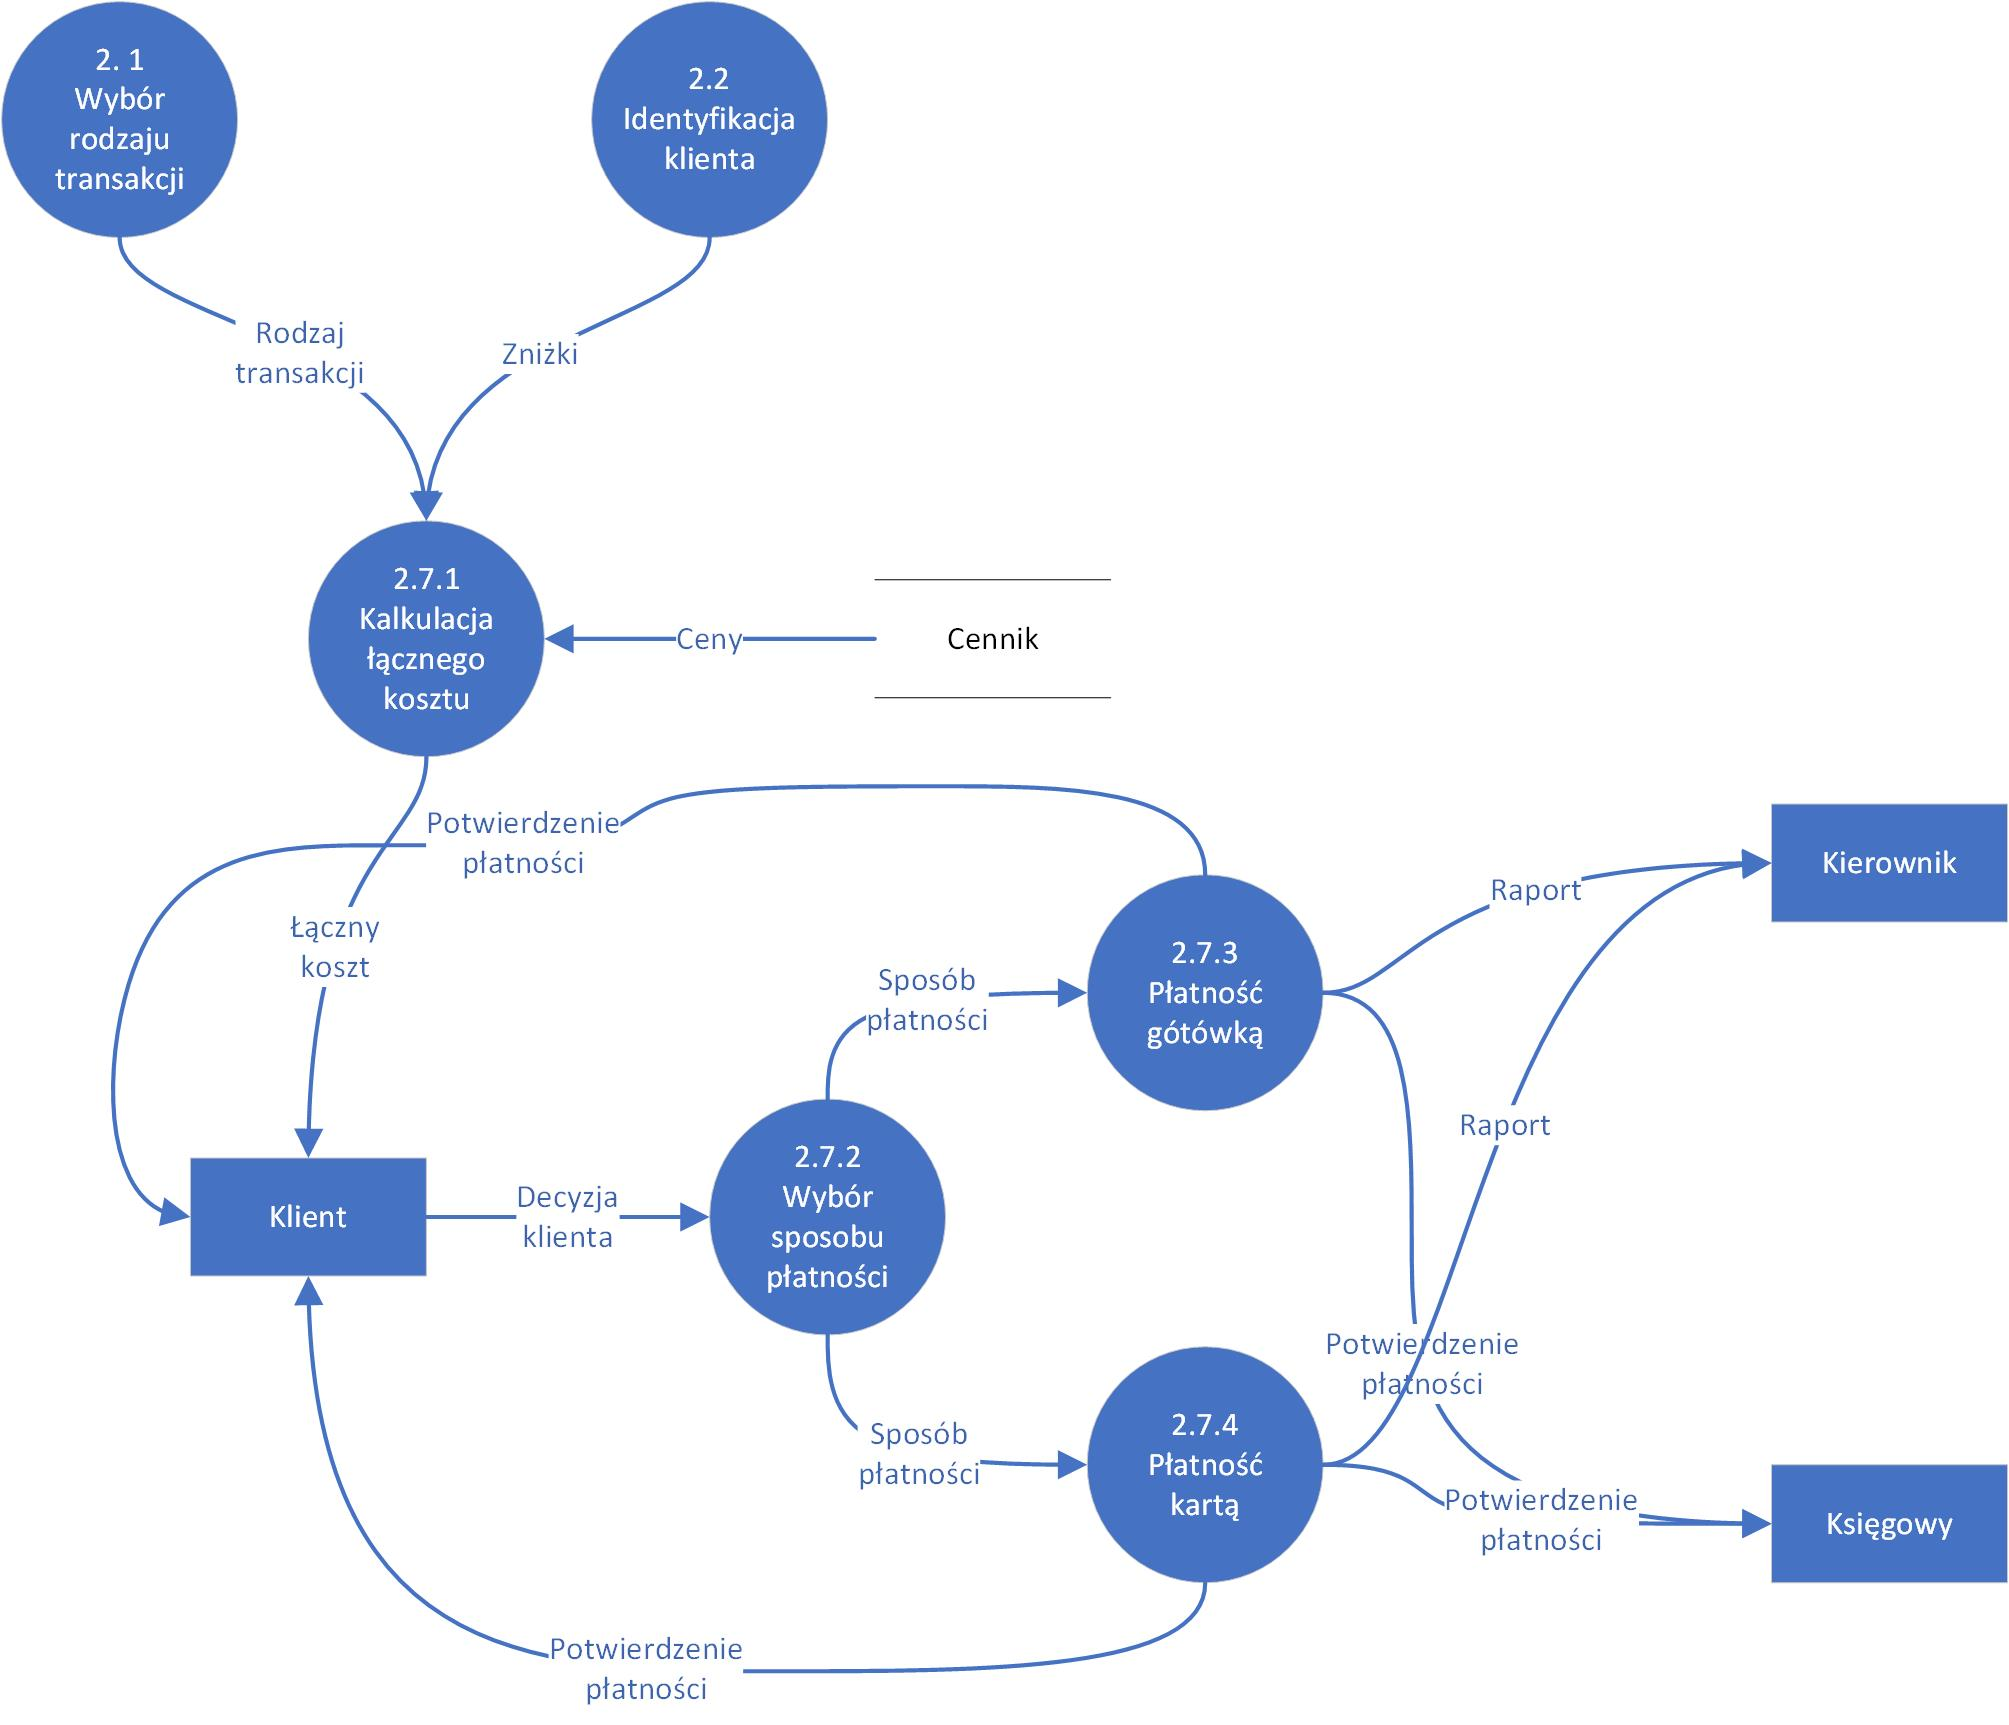
\includegraphics[scale=1]{level2_2_7.jpg}}
    \label{fig:level2_2_7}
    \end{figure}
    \newpage
    
\subsubsection{Dekompozycja procesu Wypłacanie należności}
    \begin{figure}[!htb]
    \centerline{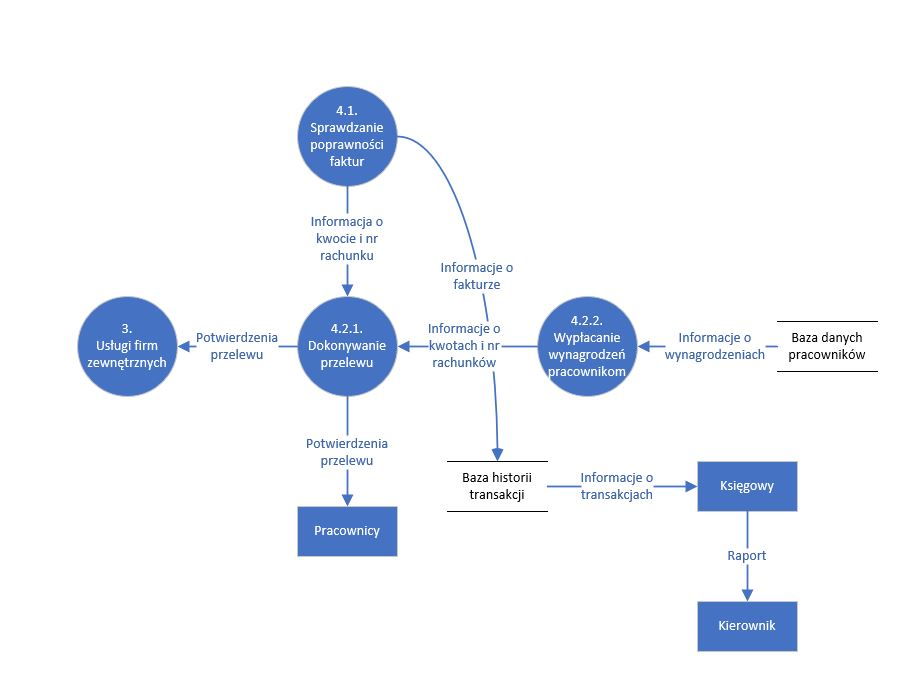
\includegraphics[scale=1.1]{level2_4_2.jpg}}
    \label{fig:level2_4_2}
    \end{figure}
    \newpage
 
\subsubsection{Dekompozycja procesu Rozliczanie podatków}
    \begin{figure}[!htb]
    \centerline{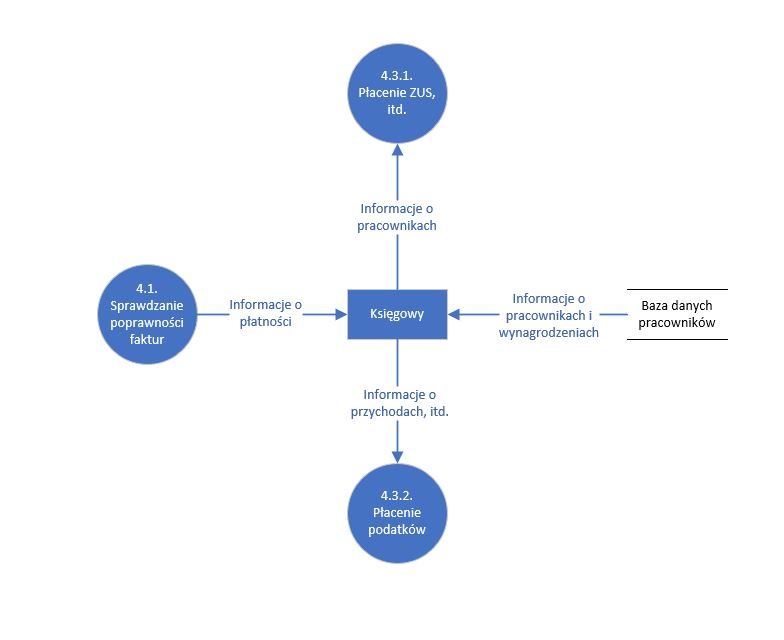
\includegraphics[scale=1.1]{level2_4_3.jpg}}
    \label{fig:level2_4_3}
    \end{figure}
    \newpage

\section{Diagram ERD}   
 \begin{figure}[!htb]
    \centerline{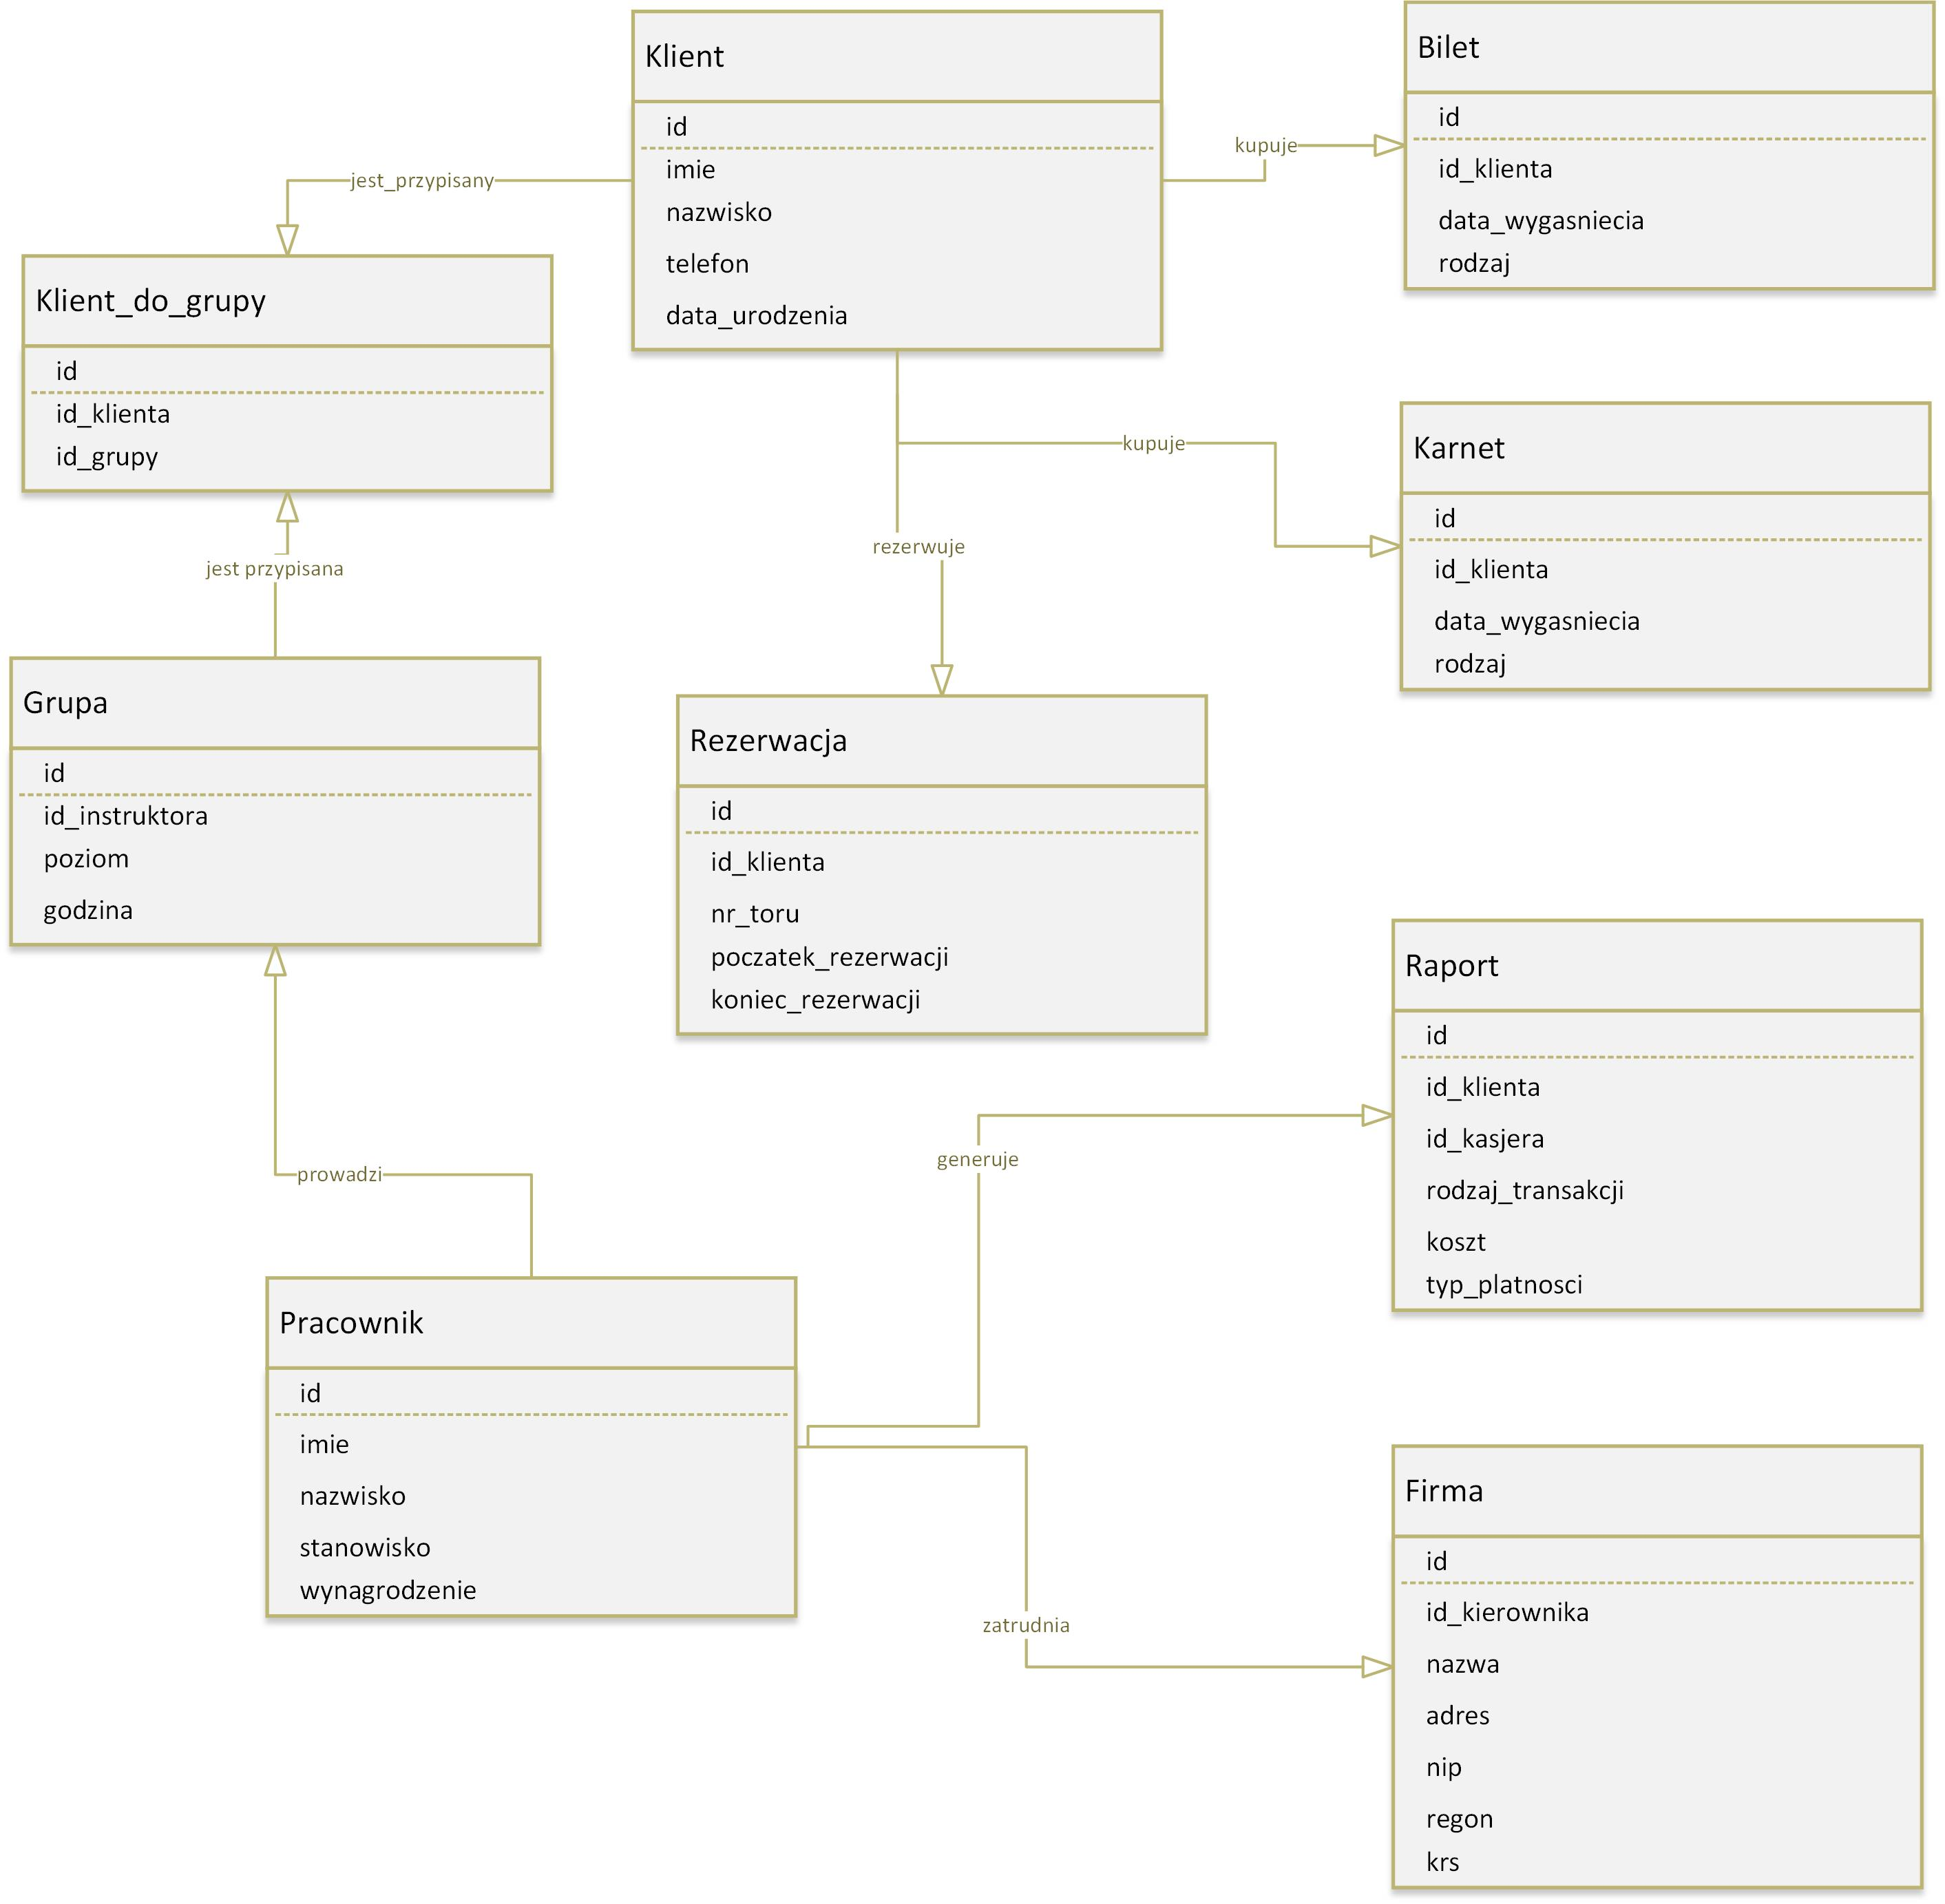
\includegraphics[scale=0.7]{erd.jpg}}
    \label{fig:erd}
    \end{figure}
    \newpage

\section{PSPEC}

\subsection{Spis procesów}
\begin{enumerate}
    \item Założenie konta
        \begin{enumerate}
            \item Weryfikacja danych klienta
                \begin{enumerate}
                    \item Sprawdzenie poprawności danych osobowych
                    \item Weryfikacja adresu email
                    \item Sprawdzenie poprawności danych płatniczych
                \end{enumerate}
            \item Zapis danych klienta do bazy
                \begin{enumerate}
                    \item Ustalenie typu konta
                    \item Generowanie raportów
                \end{enumerate}
            \item Obsługa płatności za założenie konta
                \begin{enumerate}
                    \item Generowanie potwierdzenia płatności
                \end{enumerate}
        \end{enumerate}
    \item Obsługa transakcji
        \begin{enumerate}
            \item Wybór rodzaju transakcji
            \item Identyfikacja klienta
            \item Pojedynczy bilet
                \begin{enumerate}
                    \item Wybór ilości godzin
                \end{enumerate}
            \item Karnet
                \begin{enumerate}
                    \item Wybór rodzaju karnetu
                \end{enumerate}
            \item Nauka pływania
                \begin{enumerate}
                    \item Wybór poziomu zaawansowania
                    \item Przypisanie do grupy
                \end{enumerate}
            \item Rezerwacja toru
                \begin{enumerate}
                    \item Wybór terminu rezerwacji toru
                    \item Przypisanie toru do rezerwacji
                \end{enumerate}
            \item Obsługa płatności
                \begin{enumerate}
                    \item Kalkulacja łącznego kosztu
                    \item Wybór sposobu płatności
                    \item Płatność gotówką
                    \item Płatność kartą
                \end{enumerate}
        \end{enumerate}
    \item Usługi firm zewnętrznych
        \begin{enumerate}
            \item Firma sprzątająca
            \item Firma gastronomiczna
            \item Firma obsługująca płatności
            \item Firma ratownicza
        \end{enumerate}
    \item Obsługa wynagrodzeń
        \begin{enumerate}
            \item Sprawdzanie poprawności faktur
            \item Wypłacanie należności
                \begin{enumerate}
                    \item Dokonywanie przelewu
                    \item Wypłacanie wynagrodzeń pracownikom
                \end{enumerate}
            \item Rozliczanie podatków
                \begin{enumerate}
                    \item Płacenie ZUS, itd.
                    \item Płacenie podatków
                \end{enumerate}
        \end{enumerate}
\end{enumerate}


\subsection{Opis procesów}
\begin{enumerate}
    \item \pspec {Założenie konta} {Informacje o nowym użytkowniku}{Potwierdzenie założenia konta} {Obsługuje cały proces zakładania konta}
        \begin{enumerate}
            \item \pspec{ Weryfikacja danych klienta }{Dane klienta}{Dane klienta}{Na podstawie dostarczonych danych decyduje o ich poprawności, w przypadku niepoprawności dostarcza komunikat o błędzie}
                \begin{enumerate}
                    \item \pspec{Sprawdzenie poprawności danych osobowych} {Dane osobowe} {Dane osobowe} {Na podstawie dostarczonych danych osobowych decyduje o ich poprawności (np. poprawność numeru pesel), w przypadku niepoprawności dostarcza komunikat o błędzie}
                    \item \pspec{ Weryfikacja adresu email } {Adres email} {Adres email} {Wysyła maila z kodem rejestracyjnym na podany adres i po wpisaniu tego kodu przez użytkownika przechodzi dalej}
                    \item \pspec{Sprawdzenie poprawności danych płatniczych} {Informacje płatnicze} {Dane płatnicze} {Na podstawie otrzymanych informacji płatniczych decyduje o ich poprawności, w przypadku niepoprawności dostarcza komunikat o błędzie}
                \end{enumerate}
            \item \pspec{ Zapis danych klienta do bazy} {Dane klienta} {Raport} {Dodaje użytkownika o podanych danych do bazy, zgodnie z Generowaniem raportów generuje raporty}
                \begin{enumerate}
                    \item \pspec {Ustalenie typu konta}{Dane klienta} {Informacje o typie konta} {W zależności od danych klienta ustala typ konta (np. przyznaje ulgę)}
                    \item \pspec {Generowanie raportów} {Informacje o klientach} {Raport} {Na podstawie danych o klientach z bazy generuje raport, który zostaje przesłany księgowemu i kierownikowi}
                \end{enumerate}
            \item \pspec {Obsługa płatności za założenie konta}{Dane klienta}{Potwierdzenie założenia konta}{Na podstawie otrzymanych danych firma zewnętrzna dokonuje płatności i wysyła potwierdzenie założenia konta}
                \begin{enumerate}
                    \item \pspec {Generowanie potwierdzenia płatności}{Informacja o udanej płatności}{Potwierdzenie płatności}{Na podstawie informacji o udanej płatności wysyła użytkownikowi potwierdzenie płatności (równoznaczne z potwierdzeniem założenia konta}
                \end{enumerate}
        \end{enumerate}
    \item \pspec{Obsługa transakcji}{Informacje o nowej transakcji, informacja o zmianach cen, informacja o zakończonych zajęciach}{Potwierdzenie finalizacji transakcji, Informacja o zleconych zajęciach, Informacje o zawartych trasakcjach, raport}{Na podstawie danych od klienta proces decyduje o rodzaju transakcji i przeprowadza obsługę płatności}
        \begin{enumerate}
            \item \pspec{Wybór rodzaju transakcji}{Informacje o transakcji}{Decyzja klienta}{Podjęcie decyzji o rodzaju transakcji na podstawie danych pobranych od klienta.}
            \item \pspec{Identyfikacja klienta}{Dane osobowe, Informacje o koncie}{Zniżki}{Pobranie danych klienta z bazy danych w celu określenia przysługujących zniżek.}
            \item \pspec{Pojedynczy bilet}{Decyzja klienta}{Informacje o transakcji}{Obsługa zakupu pojedynczego biletu.}
                \begin{enumerate}
                    \item \pspec{Wybór ilości godzin}{Decyzja klienta}{Informacje o transakcji}{Podjęcie decyzji o czasie ważności biletu na podstawie danych od klienta.}
                \end{enumerate}
            \item \pspec{Karnet}{Decyzja klienta}{Informacje o transakcji}{Obsługa zakupu karnetu}
                \begin{enumerate}
                    \item \pspec{Wybór rodzaju karnetu}{Decyzja klienta}{Informacje o transakcji}{Podjęcie decyzji o rodzaju karnetu (dzienny, tygodniowy, miesięczny) na podstawie danych od klienta.}
                \end{enumerate}
            \item \pspec{Nauka pływania}{Decyzja klienta}{Informacje o transakcji}{Obsługa zapisu do grupy nauki pływania.}
                \begin{enumerate}
                    \item \pspec{Wybór poziomu zaawansowania}{Decyzja klienta}{Poziom zaawansowania}{Podjęcie decyzji o poziomie zaawansowania na podstawie danych od klienta}
                    \item \pspec{Przypisanie do grupy}{Poziom zaawansowania, Informacja o wolnych miejscach}{Informacje o transakcji, Informacja o zapisie}{Zapisanie klienta do grupy z wolnymi miejscami o odpowiednim poziomie zaawanasowania.}
                \end{enumerate}
            \item \pspec{Rezerwacja toru}{Decyzja klienta}{Informacje o transakcji}{Obsługa rezerwacji toru}
                \begin{enumerate}
                    \item \pspec{Wybór terminu rezerwacji toru}{Decyzja klienta, Informacja o wolnych torach}{Termin, Wybrany tor}{Podjęcie decyzji o terminie i torze do rezerwacji na podstawie danych od klienta i danych o wolnych torach pobranych z bazy}
                    \item \pspec{Przypisanie toru do rezerwacji}{Wybrany tor}{Informacja o rezerwacji, Informacje o transakcji}{Zapis informacji o rezerwacji do bazy danych}
                \end{enumerate}
            \item \pspec{Obsługa płatności}{Informacje o płatności}{Potwierdzenie płatności, raport}{Proces odpowiadający za obsługę płatności różnymi metodami oraz utworzenie raportów dla księgowego i kierownika}
                \begin{enumerate}
                    \item \pspec{Kalkulacja łącznego kosztu}{Rodzaj transakcji, zniżki, ceny}{łączny koszt}{Proces obliczający łączny koszt transakcji zależnie od jej rodzaju, aktualnego cennika i zniżek przypadających klientowi.}
                    \item \pspec{Wybór sposobu płatności}{Decyzja klienta}{Sposób płatności}{Podjęcie decyzji o sposobie płatności na podstawie danych pobranych od klienta}
                    \item \pspec{Płatność gotówką}{Sposób płatności}{Potwierdzenie płatności, raport}{Obsługa płatności gotówkowej i utworzenie raportów i potwierdzeń płatności}
                    \item \pspec{Płatność kartą}{Sposób płatności}{Potwierdzenie płatności, raport}{Obsługa płatności kartą i utworzenie raportów i potwierdzeń płatności}
                \end{enumerate}
        \end{enumerate}
    \item \pspec{Usługi firm zewnętrznych}{Informacje o zatrudnieniu firm}{Faktura}{Zatrudnione firmy wystawiają nam faktury, które są przesyłane do Obsługi wynagrodzeń}
        \begin{enumerate}
            \item \pspec {Firma sprzątająca} {Zlecenie} {Faktura} {Firma świadczy usługi sprzątające}
            \item \pspec {Firma gastronomiczna} {Zlecenie} {Faktura} {Firma świadczy usługi gastronomiczne na terenie basenu}
            \item \pspec {Firma obsługująca płatności} {Zlecenie} {Faktura} {Firma obsługuje płatności internetowe}
            \item \pspec {Firma ratownicza} {Zlecenie} {Faktura} {Firma dba o zachowanie standardów bezpieczeństwa na basenie}
        \end{enumerate}
    \item \pspec {Obsługa wynagrodzeń} {Faktury, Informacje o zatrudnionych firmach} {Dane o wynagrodzeniach, Potwierdzenia wypłaty wynagrodzeń} {Moduł obsługuje całość wypłat wynagrodzenia}
        \begin{enumerate}
            \item \pspec {Sprawdzanie poprawności faktur}{Faktury, Informacje o zatrudnionych firmach}{Informacja o płatności (do Rozliczenia podatków), Zlecenie płatności - czyli Numer rachunku i kwota (do Wypłacania należności} {Sprawdza zgodnośc informacji na fakturach wystawionych przez firmy zewnętrzne z faktycznymi informacjami o tych firmach, zapisanymi w bazie}
            \item \pspec {Wypłacanie należności}{Zlecenie płatności, Informacje o wynagrodzeniach}{Potwierdzenie płatności, Potwierdzenia wypałaty wynagrodzeń} {Moduł obsługuje przelewy na rzecz firm zewnętrznych jak i pracowników}
                \begin{enumerate}
                    \item \pspec {Dokonywanie przelewu} {Zlecenie płatności} {Potwierdzenie płatności} {Dokonuje przelewu i dostarcza potwierdzenie płatności}
                    \item \pspec {Wypłacanie wynagrodzeń pracownikom} {Informacje o wynagrodzeniach} {Zlecenie płatności} {Pobiera informacje o wynagrodzeniach z bazy i na tej podstawie wysyła zlecenia płatności do Dokonywania przelewu}
                \end{enumerate}
            \item \pspec {Rozliczanie podatków}{Informacje o płatnościach, Informacje o pracownikach i wynagrodzeniach}{Brak}{Moduł rozlicza podatki}
                \begin{enumerate}
                    \item \pspec {Płacenie ZUS, itd.} {Informacje o pracownikach} {Brak} {Dla każdego pracownika na podstawie informacji o zatrudnieniu dokonuje rozliczenia wszystkich opłat}
                    \item \pspec {Płacenie podatków} {Informacje o przychodach i wydatkach} {Brak} {Na podstawie przychodów i wydatków dokonuje rozliczenia podatków dochodowych itd.}
                \end{enumerate}
        \end{enumerate}
\end{enumerate}
\newpage


\section{Diagramy STD}
\subsection{Zakladanie konta}
    \begin{figure}[!htb]
    \centerline{\includegraphics[scale=0.9]{zakladanie_konta.jpg}}
    \label{fig:zakladanie_konta}
    \end{figure}
\newpage
\subsection{Zakup biletu}
    \begin{figure}[!htb]
    \centerline{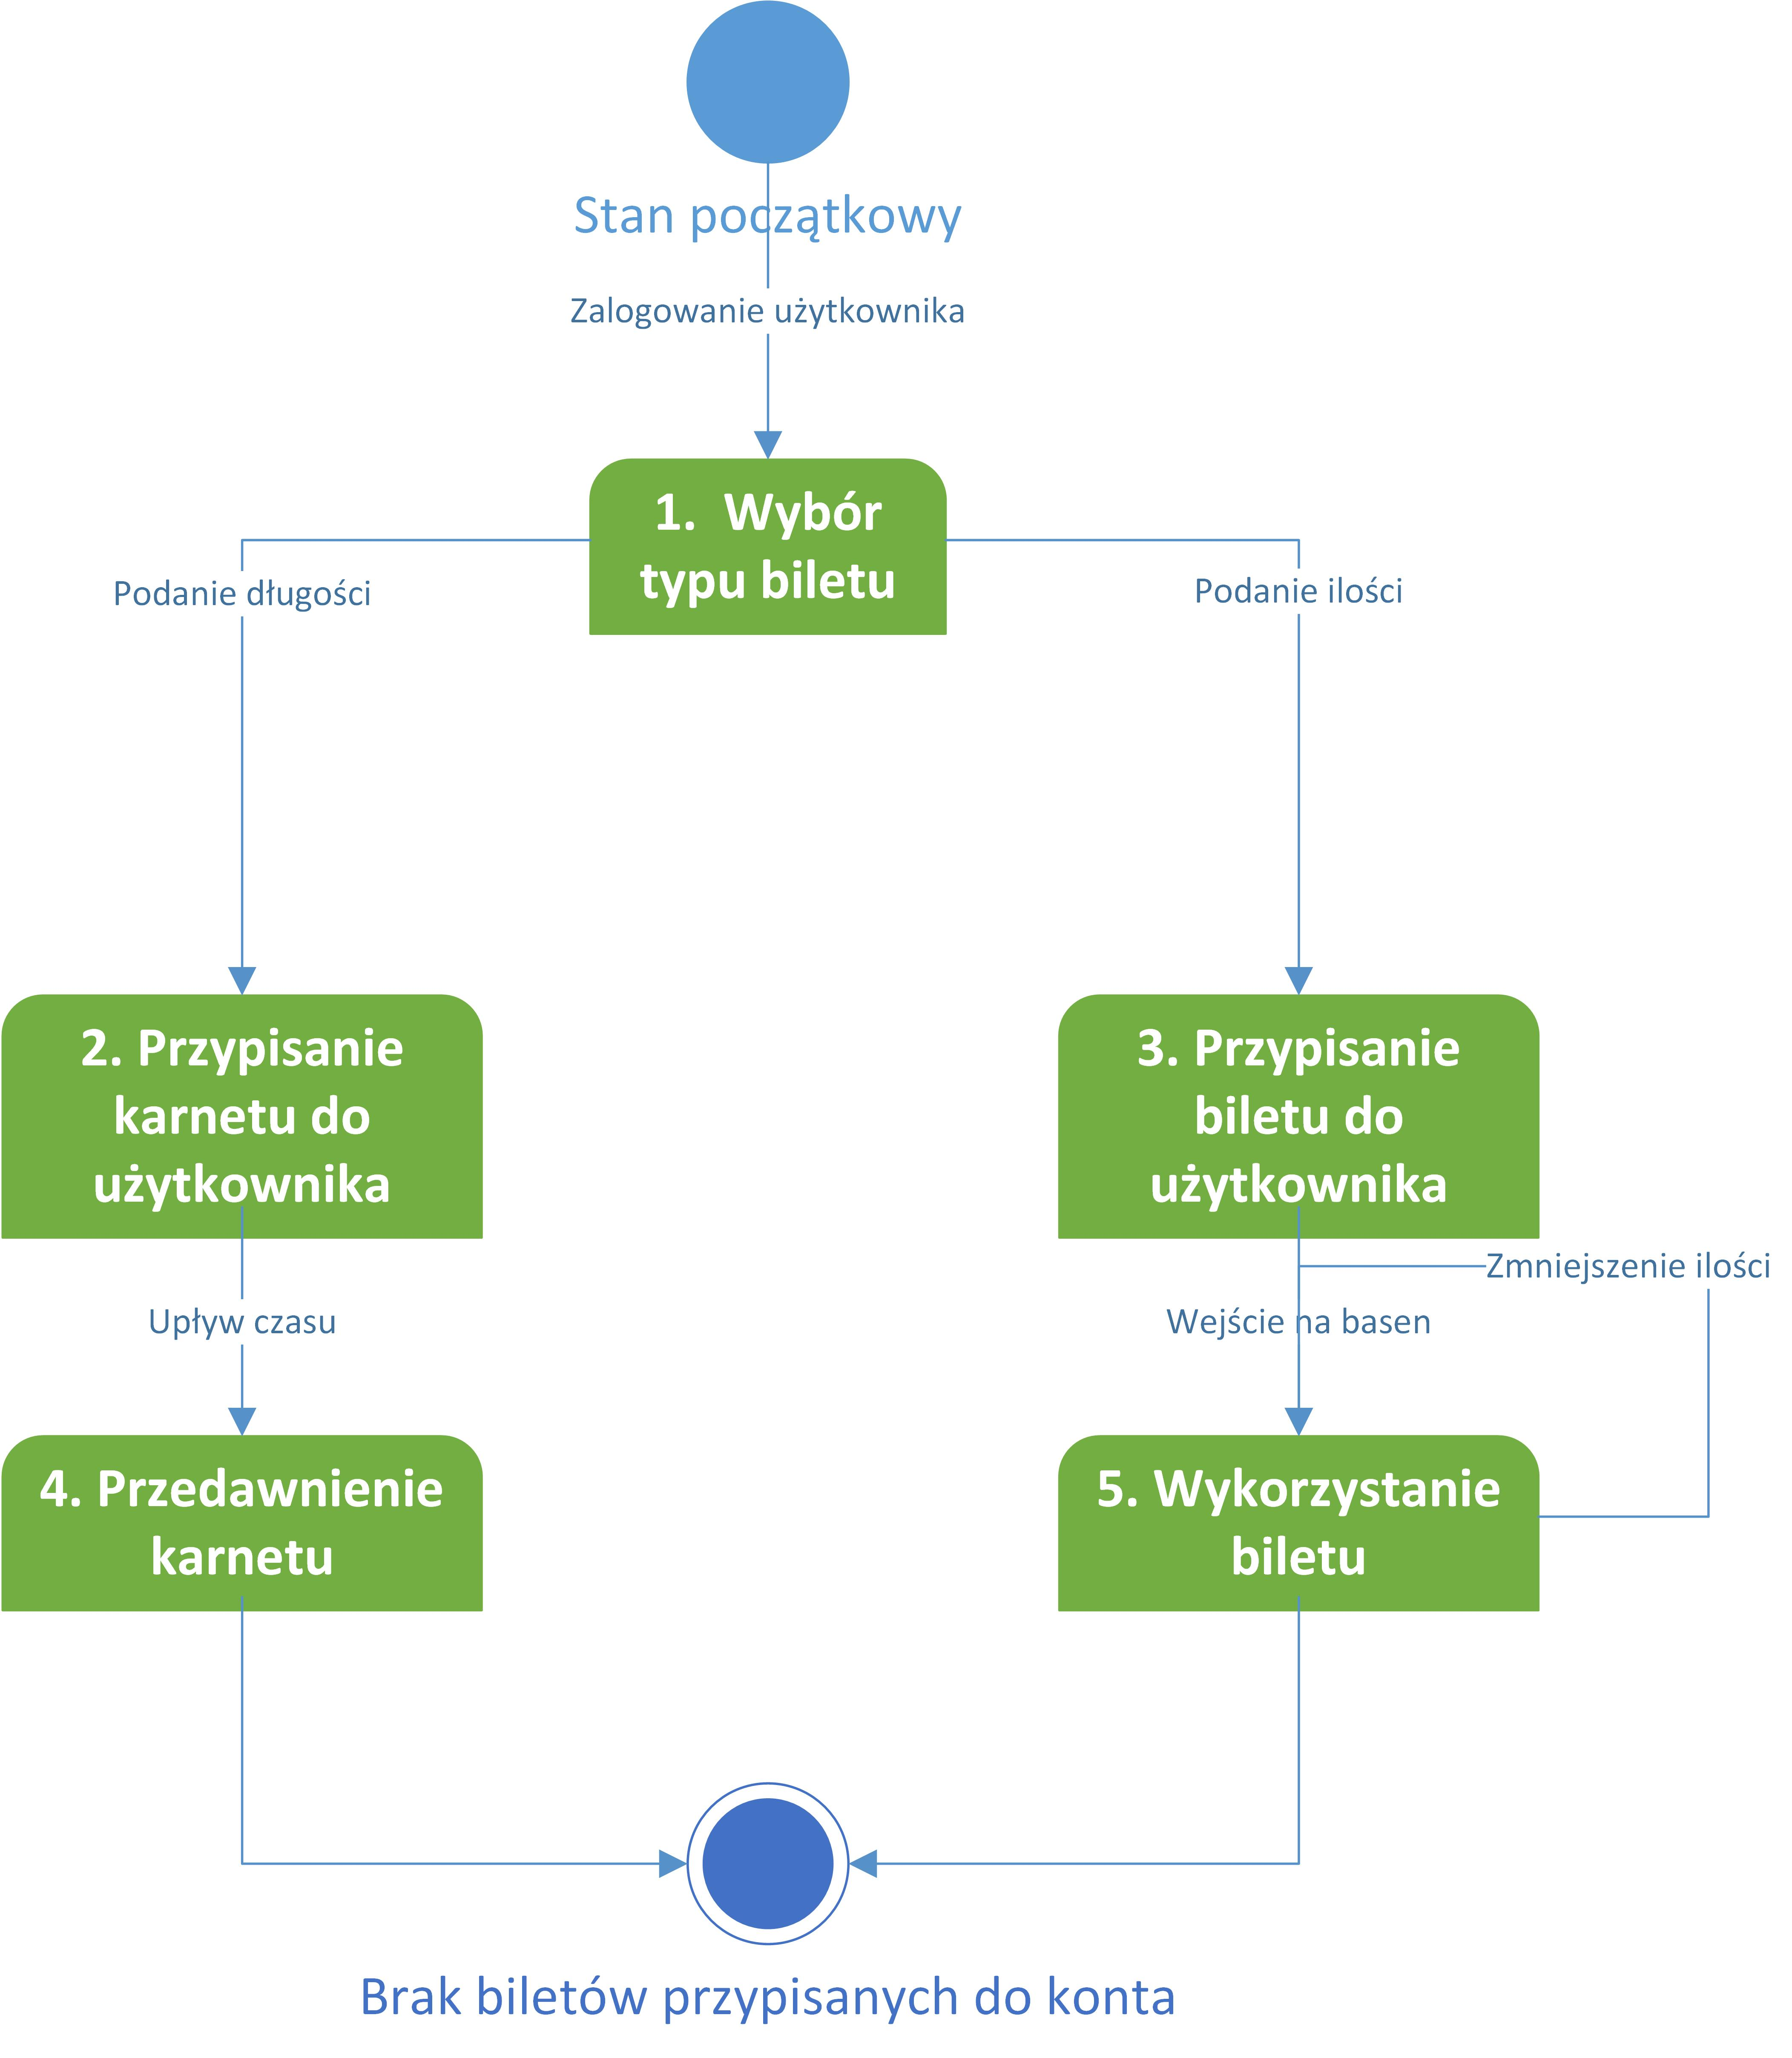
\includegraphics[scale=0.9]{zakup_biletu.jpg}}
    \label{fig:zakup_biletu}
    \end{figure}
\newpage
\subsection{Rezerwacja toru}
    \begin{figure}[!htb]
    \centerline{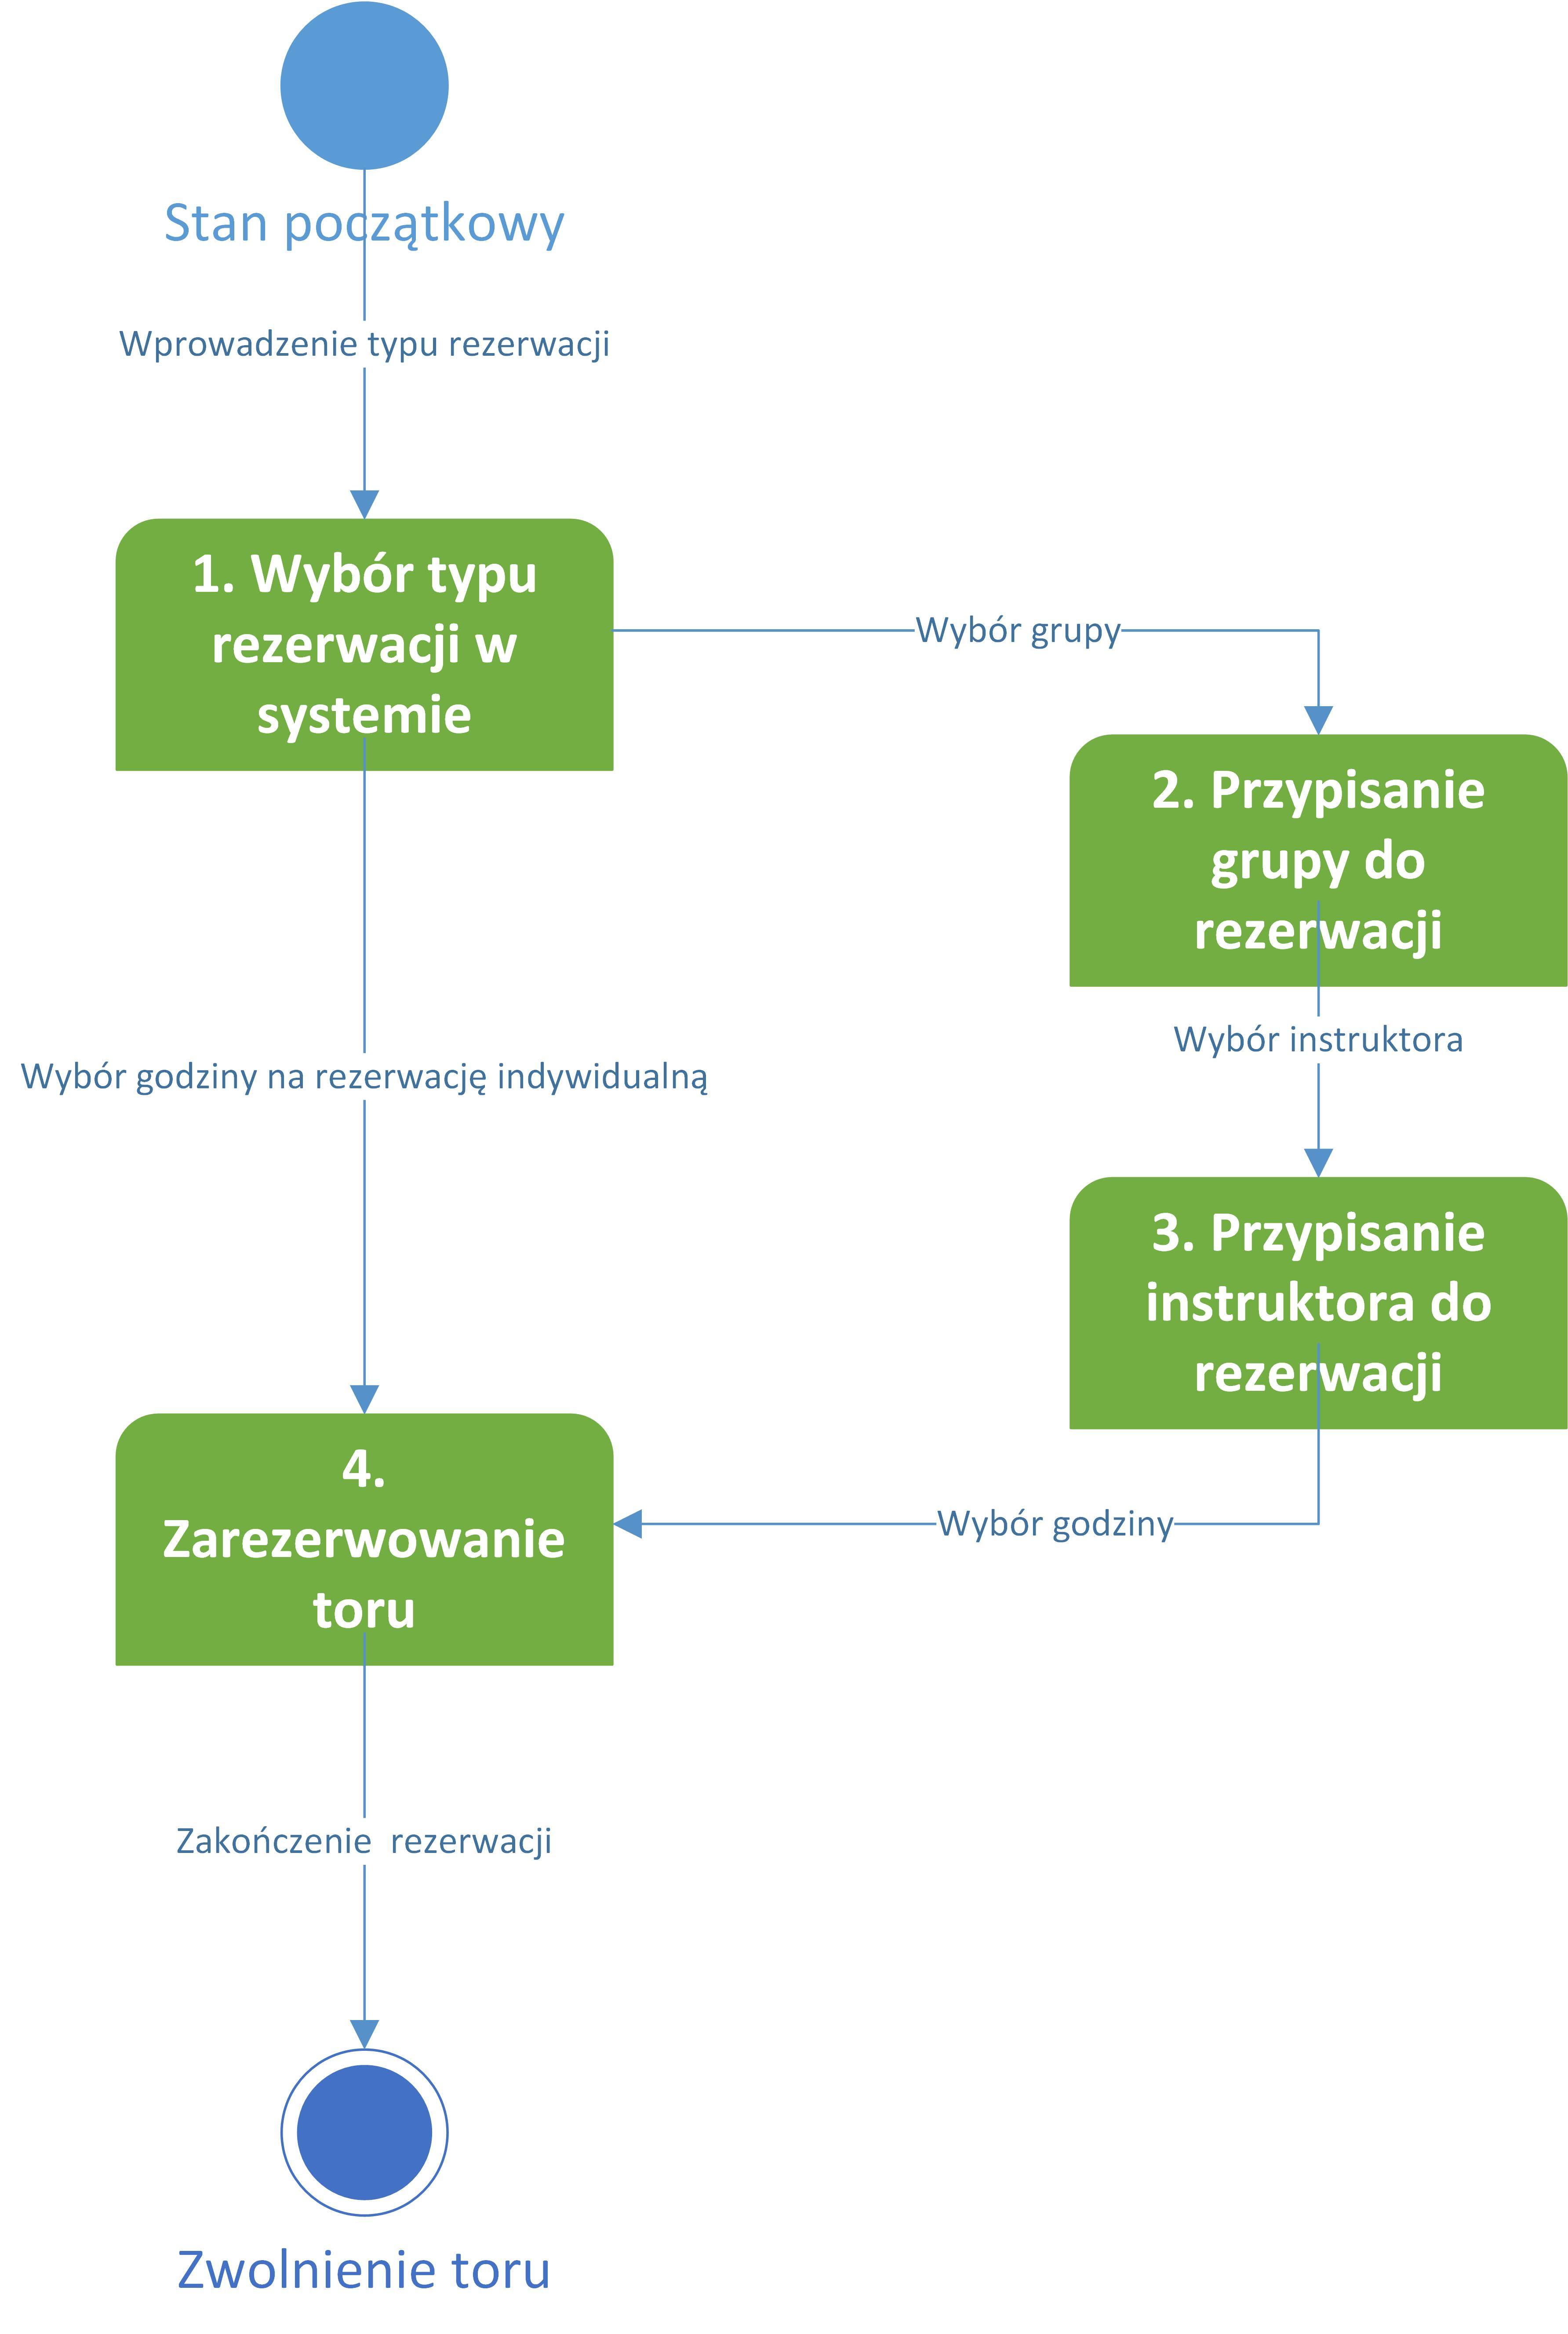
\includegraphics[scale=0.9]{rezerwacje_toru.jpg}}
    \label{fig:rezerwacje_toru}
    \end{figure}
\newpage
\subsection{Lekcje pływania}
    \begin{figure}[!htb]
    \centerline{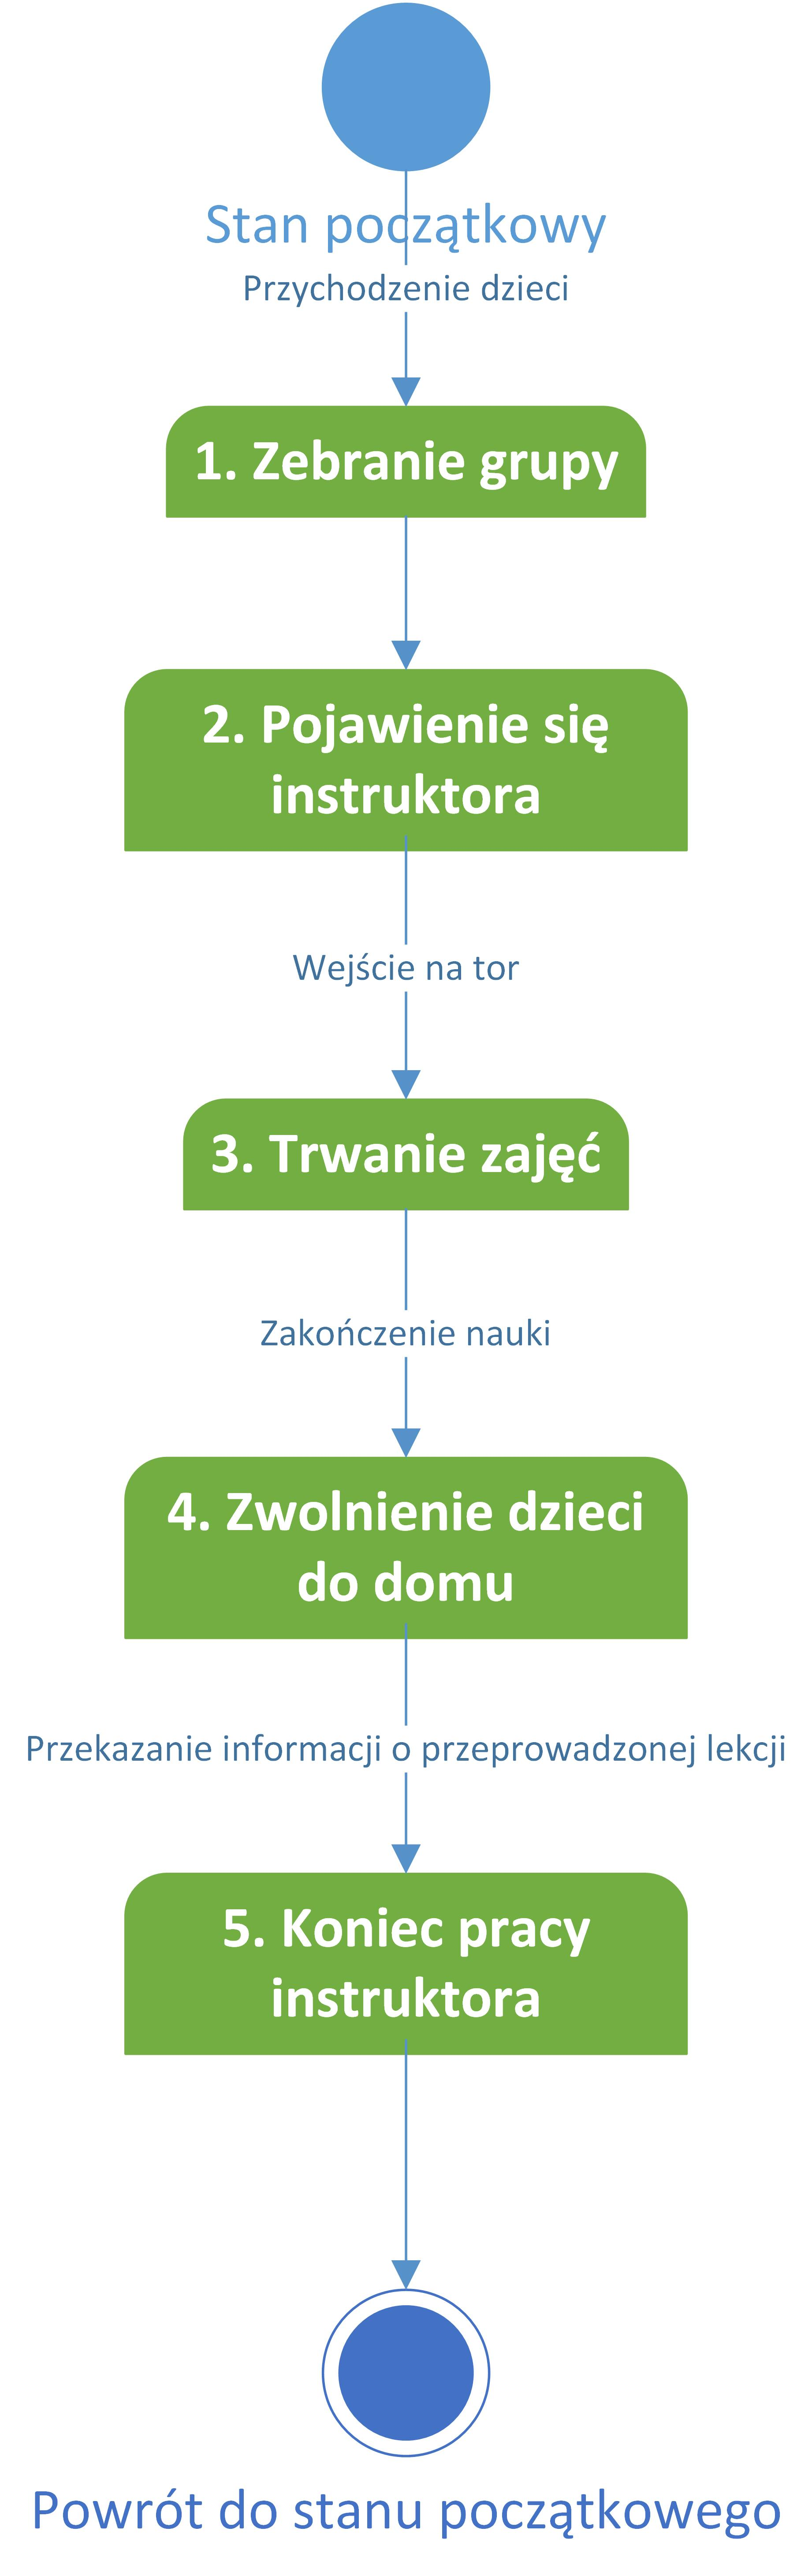
\includegraphics[scale=0.9]{lekcje_plywania.jpg}}
    \label{fig:lekcje_plywania}
    \end{figure}
\newpage


\section{Słownik Danych}
\begin{enumerate}[label= \textbf{\Alph*}]
\item \begin{itemize} %A
    \item[]
    Adres = kraj + województwo + miasto + kod pocztowy + ulica + numer domu
\end{itemize}
\item \begin{itemize} %B
    \item[]
\end{itemize}
\item \begin{itemize} %C
    \item[]
    Cena = kwota + nazwa uslugi
\end{itemize}
\item \begin{itemize} %D
    \item[]
    Dane klienta = dane osobowe + adres email + dane płatnicze
    \item[]
    Dane osobowe = imię + nazwisko + telefon + data urodzenia
    \item[]
    Dane o wynagrodzeniach = id pracownika + kwota
    \item[]
    Dane płatnicze = numer karty + kod CVC + data wygaśnięcia
\end{itemize}
\item \begin{itemize} %E
    \item[]
\end{itemize}
\item \begin{itemize} %F
    \item[]
    Faktura = kwota + id firmy + numer konta
\end{itemize}
\item \begin{itemize} %G
    \item[]
\end{itemize}
\item \begin{itemize} %H
    \item[]
\end{itemize}
\item \begin{itemize} %I
    \item[]
    Informacje o nowym użytkowniku = dane klienta
    \item[]
    Informacje o pracownikach = lista<id pracownika>
    \item[]
    Informacja o przychodach lub wydatkach = kwota + data + Przychodzący|Wychodzący
    \item[]
    Informacje o rezerwacji = nr toru + data
    \item[]
    Informacje o transakcji = kwota + konto docelowe + dodatkowe informacje
    \item[] 
    Informacje o typie konta = Normalny | Zniżki
    \item[]
    Informacja o udanej płatności = kwota + data + numer konta docelowego
    \item[]
    Informacja o wolnych miejscach = ilosc wolnych miejsc + id grupy
    \item[]
    Informacja o wolnych torach = id toru + daty rezerwacji
    \item[]
    Informacja o zapisie = id klienta + id grupy + poziom + godzina + id instruktora
    \item[]
    Informacje o zatrudnionych firmach = lista<id firmy>
    
\end{itemize}
\item \begin{itemize} %J
    \item[]
\end{itemize}
\item \begin{itemize} %K
    \item[]
    
\end{itemize}
\item \begin{itemize} %L
    \item[]
    Łączny koszt = suma cen usług
\end{itemize}
\item \begin{itemize} %M
    \item[]
\end{itemize}
\item \begin{itemize} %N
    \item[]
\end{itemize}
\item \begin{itemize} %O
    \item[]
\end{itemize}
\item \begin{itemize} %P
    \item[]
    Potwierdzenie płatności = mail z informacją o udanej płatności
    \item[]
    Potwierdzenie wypłaty wynagrodzenia = mail z kwotą, id pracownika i numerem konta
    \item[]
    Potwierdzenie założenia konta = plik pdf z danymi użytkownika i datą
    \item[]
    Poziom zaawansowania = 1|2|3|4|5|Nieznany
\end{itemize}
\item \begin{itemize} %Q
    \item[]
\end{itemize}
\item \begin{itemize} %R
    \item[]
    Raport = plik pdf z informacjami o użytkownikach | przychodach | wydatkach
\end{itemize}
\item \begin{itemize} %S
    \item[]
    Sposób płatności = karta przy kasie | gotówka przy kasie | przelew | Przelewy24
\end{itemize}
\item \begin{itemize} %T
    \item[]
\end{itemize} 
\item \begin{itemize} %U
    \item[]
\end{itemize}
\item \begin{itemize} %V
    \item[]
\end{itemize}
\item \begin{itemize} %W
    \item[]
    Wybrany tor = id toru
\end{itemize}
\item \begin{itemize} %X
    \item[]
\end{itemize}
\item \begin{itemize} %Y
    \item[]
\end{itemize}
\item \begin{itemize} %Z
    \item[]
    Zlecenie = cena + id firmy + opis usługi
    \item[]
    Zniżki = 20\%|10\%
\end{itemize}
\end{enumerate}
 
 
\end{document}
